% The manuscript body, shared by both front ends (paper.tex, emse/main.tex):
% Introduction through Conclusion, Future Work and the Carbon Footprint section.
% Generated tables are read through \gendir, which each front end defines.
% Detail cut from the article lives in appendix.tex: Online Resource 1 for EMSE
% (emse/esm.tex), an inline appendix for Elsevier. \esmsec, \esmtab, \esmfig and
% \ESMname phrase a pointer to it for whichever front end is building.
%%%%%%%%%%%%%%%%%%%%%%%%%%%%%%%%%%%%%%%%%%%%%%%%%%%%%%%%%%%%%%%%%%%%%%%%%%%%%%%
\section{Introduction}
\label{sec:intro}

The rapid advancement of Artificial Intelligence (AI), particularly Deep Learning (DL), has delivered progress across domains such as healthcare, natural language processing, environmental monitoring and autonomous systems, at a growing environmental cost: training and deploying state-of-the-art neural networks demands vast computational resources and energy~\citep{strubell2019energy,lacoste2019quantifying,bender2021stochastic,xu2021survey,patterson2021carbon,luccioni2023counting,kaack2022aligning}.
Energy use and emissions vary widely with model architecture, dataset size, hardware infrastructure and even the geographic location of execution~\citep{patterson2022plateau,luccioni2022bloom}; standardized benchmarks such as MLPerf Tiny have begun to incorporate energy measurements~\citep{banbury2021mlperf}; and sustainability has become a central dimension of AI research~\citep{henderson2020systematic,schwartz2020green}.

The field has responded with \emph{Green AI}~\citep{schwartz2020green,verdecchia2023systematic}, which promotes AI systems that are energy-conscious as well as accurate. Surveys report advances in lightweight architectures, efficient training and inference, model compression and hardware-aware optimisation~\citep{xu2021survey,mehlin2023towards,tripp2024measuring,yarally2023uncovering}, and evidence increasingly suggests that energy improvements need not degrade accuracy~\citep{cruz2025greening}.

Beyond algorithmic efficiency, research in software sustainability has shown that the choice of programming language itself can have a substantial impact on energy usage~\citep{pereira2021ranking,georgiou2017analyzing,pereira2017energy,gordillo2024ranking,chandra2019impact,mahadevappa2021energy,maleki2017understanding}, and on the run time and memory that partly determine it~\citep{nanz2015comparative}. Nevertheless, while both Green AI and the environmental sustainability of programming languages have been independently investigated, their intersection remains largely unexplored.
A first step was made by \citet{georgiou2022green}, who analyzed the energy footprint of Deep Learning frameworks within Python, and by \citet{marini2025green}, who studied the impact of programming languages in AI workloads and state explicitly that they ``purposely opted not to focus on GPU-intensive algorithms such as deep neural networks, leaving their consideration as future work''. That is the gap this study addresses.

For a practitioner, however, a programming language is inseparable from its \emph{ecosystem}: choosing a language for DL implies adopting a software stack of bindings, frameworks, runtimes and driver/toolchain dependencies. In real-world settings it is therefore more meaningful to evaluate \emph{language--framework ecosystems} as they are adopted in practice than to isolate a ``pure'' language effect under synthetic conditions.

Prior work has approached this from three directions without closing it. Energy has been compared across DL frameworks \emph{within} one language ecosystem, including at the GPU and runtime-infrastructure level~\citep{georgiou2022green,alizadeh2024energy}; language-level energy has been measured for CPU-bound general-purpose workloads~\citep{pereira2021ranking,gordillo2024ranking}; and the \emph{runtime} cost of cross-language DL bindings has been characterised for time, memory and accuracy, but not for energy~\citep{li2024bindings}. What has not been measured is energy across multiple language-based DL stacks for GPU training and inference, where frameworks, execution engines, toolchains and dataset complexity all vary together~\citep{weber2023twins}.

This paper addresses this gap with an empirical study of \emph{the impact of language--framework ecosystems on the energy efficiency of DL workloads}: two widely adopted convolutional neural networks (ResNet-18 and VGG-16) across \vEcosystems{} ecosystems, spanning five host languages (Python, C++, Java, R and Rust) and the frameworks each offers in practice (PyTorch, TensorFlow and JAX; LibTorch; Deeplearning4j; the \texttt{torch} and \texttt{tch} bindings), on three datasets (Fashion-MNIST, CIFAR-100 and Tiny ImageNet), with one declared contrast cell on Imagenette at $224\times224$ and batch 32 that raises per-sample compute.

A cross-ecosystem energy comparison, however, rests on two premises that are rarely stated and never visible in the resulting numbers: that every stack is running the same experiment, and that every stack is measured the same way. We found both far harder to satisfy than the literature suggests. An earlier campaign of ours, of exactly this shape, was executed carefully and produced an entirely coherent story; auditing it against its own source code afterwards showed that the stacks had drifted apart in learning rate, input shape, evaluation batching and data-loader parallelism, that the measurement tool had been configured five different ways across them, and that two stacks were capable of running the whole workload on the CPU while reporting nothing but a log line. None of this was visible in the energy figures. All of it moved them.

We therefore treat the apparatus as part of the contribution rather than as a preliminary, with three commitments. \emph{(i)} A written experiment specification states what ``the same experiment'' means across stacks, and \vConformanceChecks{} automated checks enforce it against the source code, so that a divergence fails a check instead of quietly changing a number. \emph{(ii)} Energy is read from hardware counters, NVML's accumulated-energy register for the accelerator and the RAPL package-energy counters for the CPU, with CodeCarbon running over the same phase boundaries as a second reading. \emph{(iii)} Each configuration is executed as \vRepetitions{} independent, interleaved runs with distinct seeds, so that the run rather than the epoch is the unit of analysis, and every ecosystem records per-epoch test accuracy, so that energy can be normalised by the quality actually reached.

Our results are correspondingly more modest and more defensible than a bare ranking. Under a common measurement boundary, and with a median between-run coefficient of variation of \vCVTrainMedian\,\%, training energy differs across ecosystems by \vSpreadTrainMin$\times$ to \vSpreadTrainMax$\times$; final test accuracy converges to within \vAccBlockSpreadFashionMax{} percentage points on Fashion-MNIST but not on the two harder datasets, where energy must be read alongside quality. In the $224\times224$ contrast cell the spread among the six stacks other than Java falls to \vSatNoJavaSpreadTrainResnet$\times$ and \vSatNoJavaSpreadTrainVgg$\times$, while Java, which reaches no cuDNN kernel, moves further away. Replication also exposed a defect we had misread as an ecosystem property: \vCollapseFirstVgg{} of \vCollapseFirstVggRuns{} VGG-16 runs of a first execution sat at chance accuracy for the whole budget because of framework weight initialisers (Section~\ref{subsubsec:collapse}). And the two readings agree on \emph{energy} to \vCCmeasDisagreementPct\,\% over \vBlocks{} blocks, because on this platform the estimator reads the same registers we do, but not on time: \vWindowPaddedPct\,\% of blocks carry seconds of tracker lifetime in the duration CodeCarbon reports, so power derived from its fields is understated by up to \vPowerUnderstatedWorst$\times$ on the shortest blocks --- a bias that lands on the fastest ecosystems and on inference, precisely the comparisons such a study exists to make.

The contributions of this work are as follows:
\begin{itemize}
    \item A systematic empirical comparison of DL energy consumption across \vEcosystems{} language--framework ecosystems for GPU-based workloads, replicated \vRepetitions{} times per configuration and reported with between-run uncertainty and quality normalisation, together with a declared contrast cell that tests how the spread changes when a higher resolution raises per-sample compute;
    \item An experiment specification for cross-ecosystem energy studies, together with \vConformanceChecks{} executable conformance checks that verify it against the source, the built binaries and the campaign's own metric files, and a single measurement contract implemented by all \vEcosystems{} stacks;
    \item A dual-instrument characterisation of CodeCarbon against hardware energy counters over \vBlocks{} measurement blocks, including a quantified failure mode of its reported duration that invalidates energy--time analyses built on it;
    \item A comprehensive replication package, including all data, scripts, and settings required to fully reproduce our results.\footnote{Replication package: \url{https://github.com/Pampaj7/DeepGreen}. The
Zenodo record \url{https://zenodo.org/records/17734884} archives the earlier
campaign and is superseded by this one.}
\end{itemize}

Detail the argument does not need --- the full specification, supplementary analyses for RQ1, RQ3 and RQ4, an illustrative industrial scenario, the complete defect catalogue and the extended threats to validity --- is in \ESMname.

%%%%%%%%%%%%%%%%%%%%%%%%%%%%%%%%%%%%%%%%%%%%%%%%%%%%%%%%%%%%%%%%%%%%%%%%%%%%%%%
\section{Background}
\label{sec:background}

\emph{Green AI}~\citep{schwartz2020green,verdecchia2023systematic,cruz2025greening}
promotes AI systems that are energy-efficient as well as accurate.
Sustainability can be quantified as carbon footprint, financial cost or energy
use~\citep{kaack2022aligning,patterson2021carbon}; we focus on \textbf{energy
consumption} in Joules, a direct and reproducible measure of computational
effort that, unlike carbon footprint, does not depend on the energy mix and
location of execution and so compares consistently across heterogeneous DL
stacks under a uniform protocol.

We treat execution time as a secondary metric, not a proxy for energy. The
prevailing position in the software-energy literature, built largely on
CPU-bound benchmarks, is that lower runtime does not imply lower
energy~\citep{weber2023twins,rua2024large,pereira2021ranking}, and 
\citet{vankempen2025green} argue that much of the reported language effect
is an artefact of how such comparisons are constructed. Our argument is
adjacent: theirs concerns confounds in what is compared, ours a field of the
instrument's output. We test the relation for a GPU-bound workload in
Section~\ref{subsec:rq3}, where the answer depends on which field of the
instrument's output is read as the duration.

\textbf{Deep Learning workloads} divide into \emph{training}, iterative
parameter updates through backpropagation, and \emph{inference}, forward passes
on a trained model; their energy profiles differ and optimisations in one do
not necessarily carry over to the other~\citep{mehlin2023towards,tripp2024measuring},
so we analyse them separately.

\textbf{Language--framework ecosystems} may influence energy through execution
engines, runtime overheads, input pipelines, precision policies and the
driver/toolchain. In GPU-based DL most computation is delegated to optimised
backend kernels, so differences should be read at the \emph{ecosystem level}
rather than attributed to the language alone; some ecosystems add runtime
layers, and this study does not attribute its measured spread to that mechanism
(Section~\ref{subsec:rq1}). Language choice, often treated as secondary,
constrains the frameworks, runtimes and toolchains available, and with them the
energy profile.

\textbf{Energy measurement} for workloads of this kind can be read at three
places, and the choice of place matters more than the choice of tool.
A \emph{wall meter} sees the whole machine including power supply losses, fans
and drives. \emph{Hardware energy counters} --- NVML's
\texttt{nvmlDeviceGetTotalEnergyConsumption} on NVIDIA accelerators and RAPL on
the CPU package, which AMD exposes as well and Linux presents under
\texttt{intel-rapl} names whatever the vendor --- accumulate energy in the
silicon itself and are read by software but not estimated by it.
\emph{Software estimators} such as \texttt{CodeCarbon}~\citep{codecarbon} sit on
top of whatever the platform exposes and substitute a model wherever it exposes
nothing.

Software estimators have become standard in sustainability-oriented AI
research~\citep{dodge2022efficient,patterson2022plateau} and are the sole
instrument in model compression analysis~\citep{paula2025comparative},
optimizer efficiency benchmarks~\citep{almog2025optimizer}, large-scale
evaluations of Large Language Models~\citep{luccioni2024power} and cybersecurity
systems~\citep{cybergreen2026} --- studies whose conclusions inherit whatever the
estimator gets wrong. Run alongside hardware wattmeters, CodeCarbon tracks
sensor readings closely under controlled conditions and deviates more on
heterogeneous infrastructure~\citep{aquino2025energyindex,bouza2023carbonfootprint};
validation against external ground truth across hundreds of AI experiments
reports errors of up to 40\%, and systematic underestimation of 20--30\% in some
settings~\citep{fischer2026groundtruthing}.

That literature asks whether an estimator's number is close to the truth; we
ask whether a study can tell when it is not. A correction factor fixes
inaccuracy, but not an estimator that silently substitutes a model for a
measurement, or pads a duration it reports as measured. We therefore instrument every measurement block
\emph{twice}: hardware counters as the primary instrument, and
\texttt{CodeCarbon} started and stopped at the same phase boundaries as a
second reading. Agreement is then an observable property of each block rather
than an assumption, and where the two cannot agree --- CodeCarbon's RAM term is
derived from installed memory capacity, and no counter on this platform can
confirm or refute it --- the gap is identified rather than absorbed. NVML plus
RAPL is a \emph{board-and-package} measurement: the accelerator card including
its memory, plus the CPU package, excluding the power supply, fans, drives and
host DRAM. We had no wall meter and report that boundary consistently rather
than a mixture of measured and modelled terms that corresponds to no physical
boundary at all; Section~\ref{sec:instrument} reports what the two instruments
say about each other.

%%%%%%%%%%%%%%%%%%%%%%%%%%%%%%%%%%%%%%%%%%%%%%%%%%%%%%%%%%%%%%%%%%%%%%%%%%%%%%%
\section{Related Work}
\label{sec:related}

Prior work compares energy across DL frameworks within one language, across
languages without deep learning, or across language bindings without energy.
\esmtab{tab:related} places this study against the nine studies closest to it
on the two axes that matter here, how many language ecosystems are compared and
how energy is measured: each of them stays within
Python~\citep{li2016evaluating,georgiou2022green,alizadeh2024energy}, leaves
deep learning out~\citep{pereira2021ranking,gordillo2024ranking,chattaraj2025rvspython},
measures no energy~\citep{li2024bindings}, compares instruments rather than
stacks~\citep{jay2023experimental}, or relies on a software estimator in a single
run~\citep{marini2025green}. This study compares \vEcosystems{} stacks across
five languages with NVML and RAPL counters, the estimator alongside, over
\vRepetitions{} runs per configuration.

Two of these deserve more than a row. \citet{alizadeh2024energy}
compare runtime infrastructures for the same models on the same GPU, and reach
the ecosystem-level question from inside Python: their treatment is the runtime
beneath one language, ours is the language--framework stack above it. 
\citet{li2024bindings} compare TensorFlow and PyTorch bindings across five
languages, which is our independent variable exactly, and measure run time,
memory and accuracy rather than energy --- the gap this study fills, and the
reason we treat the measurement boundary as a contribution rather than a
preliminary.

\citet{jay2023experimental} compare software power meters, CodeCarbon
among them, against physical meters on CPU and GPU, and establish that a
measurement window must comfortably exceed a \emph{sampling} meter's interval.
We report that our own design does not exhibit that constraint, and why: on this
platform the estimator reads accumulating registers rather than sampling, and
its energy residual against those registers is flat across every block length
(Section~\ref{sec:instrument}). What we add is orthogonal --- a characterisation
of the \emph{duration} an estimator reports beside its energy, which to our
knowledge has not been examined.

%%%%%%%%%%%%%%%%%%%%%%%%%%%%%%%%%%%%%%%%%%%%%%%%%%%%%%%%%%%%%%%%%%%%%%%%%%%%%%%
\section{Research Methodology}
\label{sec:methodology}

This work adopts an empirical methodology grounded in the principles of software engineering empirical experimentation~\citep{feldt2010validity,ampatzoglou2019identifying,sjoberg2023construct,verdecchia2023threats}.
Our objective is not to propose a new algorithm or framework, but to systematically analyze how choosing among language--framework ecosystems (including their supported runtime and toolchain) can impact the energy efficiency of DL workloads.
To this end, we designed an \textit{in vitro} controlled experiment that treats ecosystems as independent variables, DL workloads as experimental objects, and energy consumption as the primary dependent variable~\citep{basili1994gqm,cook1979quasi,campbell1963experimental}.

\textbf{Research goal and questions.}
Following the Goal-Question-Metric (GQM) paradigm~\citep{basili1994gqm}, our goal is formulated as:
\begin{quote}
    \emph{Analyze} DL training and inference, \\
    \emph{for the purpose of} quantifying and comparing their energy consumption, \\
    \emph{with respect to} the choice of DL ecosystems (i.e. language bindings, frameworks/libraries, supported runtimes/execution engines, and associated toolchains), \\
    \emph{from the viewpoint of} software engineering researchers and practitioners, \\
    \emph{in the context of} computer vision image classification workloads.
\end{quote}

\textbf{Research questions.}
This study investigates how language--framework ecosystem selection influences the energy efficiency of Deep Learning (DL) workloads.
We ask four questions:

\begin{itemize}
    \item \textbf{RQ1:} \textit{How does language--framework ecosystem choice affect the energy efficiency of DL \emph{training}?}
    \item \textbf{RQ2:} \textit{How does language--framework ecosystem choice affect the energy efficiency of DL \emph{inference}?}
    \item \textbf{RQ3:} \textit{How do energy efficiency and execution time relate across different DL ecosystems?}
    \item \textbf{RQ4:} \textit{To what extent are the answers to RQ1--RQ3 determined by the measurement apparatus rather than by the ecosystems?}
\end{itemize}

RQ4 is not a robustness check appended to the other three. A cross-ecosystem
energy comparison is an inference from an instrument to a claim about software,
and the inference is only as good as the guarantee that the instrument reads the
same quantity, over the same window, for every stack. We therefore treat the
apparatus as an object of measurement in its own right: every block is recorded
twice over the same boundaries, and RQ4 asks what those readings say about each other and
about the answers to RQ1--RQ3.

\textbf{Objects of study.}
We study two canonical convolutional architectures, ResNet-18~\citep{he2015resnet}
and VGG-16~\citep{simonyan2014vgg}, chosen for their distinct computational
characteristics (residual connections vs.\ sequential depth) and above all
because nearly every DL framework ships them \emph{off-the-shelf}, so that our
measurements capture each framework's own implementation rather than a
reimplementation of ours~\citep{xu2021survey,mehlin2023towards,tripp2024measuring}.

To account for varying workload complexity, we employ three widely utilized datasets.
\emph{Fashion-MNIST} provides a lightweight baseline with 28$\times$28 grayscale images across 10 classes~\citep{xiao2017fashion}, and is often used as a modern drop-in replacement for MNIST\footnote{\url{https://github.com/zalandoresearch/fashion-mnist}}. It includes 60,000 training and 10,000 test images.
\emph{CIFAR-100} increases complexity with 32$\times$32 color images across 100 categories, remaining a canonical benchmark for image classification~\citep{krizhevsky2009learning}, and comprises 50,000 training and 10,000 test images.
\emph{Tiny ImageNet} represents a demanding workload with 64$\times$64 color images across 200 classes and 100,000 training and 10,000 test images, serving as a proxy for ImageNet-scale tasks~\citep{le2015tinyimagenet}.

All datasets are resized once, offline, to a uniform $32\times32$
(\texttt{scripts/normalise\_dataset\_resolution.py}), so each stack's own resize
is a no-op and no framework's resampling filter can enter the comparison. Before
the change, \vPixelDivergentStacks{} of the \vEcosystems{} stacks decoded
measurably different pixels on Tiny ImageNet --- the one dataset that has to be
downsampled --- with means that agreed and variances that did not. A common
resolution preserves the datasets' differences in colour, class count and size
while removing input resolution as a confound~\citep{marini2025green,georgiou2022green},
keeps the classification layer fixed across datasets, reflects how canonical
models are reused in practice~\citep{cruz2025greening,verdecchia2023systematic},
and suits frameworks such as \texttt{tch} and Deeplearning4j that are more
reliable at standardised sizes~\citep{pereira2021ranking,gordillo2024ranking}.
It may interact with framework-specific memory and kernel selection, and at that
resolution per-sample compute is small: over the training blocks
\vSatRefUtilVggHighCount{} of the \vEcosystems{} stacks hold the accelerator at
or above \vSatRefUtilHighPct\,\% utilisation on VGG-16, but
\vSatRefUtilResnetHighCount{} on ResNet-18. We therefore ran one additional
experiment rather than extrapolate: a contrast cell on ten ImageNet classes at
$224\times224$ and batch 32, declared in the specification as S7 and reported in
Section~\ref{sec:saturation}. It changes resolution, batch size and dataset
together, and is one point, not a sweep over any of them.

\textbf{Independent and dependent variables.}
Our primary independent variable is the \emph{DL ecosystem}, i.e. the language--framework stack as adopted in practice (including its officially supported runtime and CUDA/cuDNN toolchain). In our design, each ecosystem is treated as a single categorical treatment; we do not attempt to decompose effects into separate contributions of language, framework, runtime, or toolchain.
Specifically, we evaluate \vEcosystems{} language-based ecosystems: Python (\texttt{PyTorch}, \texttt{TensorFlow}, \texttt{JAX}), C++ (\texttt{LibTorch}), Java (\texttt{Deeplearning4j}), R (\texttt{torch}), and Rust (\texttt{tch}).
A second independent variable is the \emph{DL phase} (training and inference).

MATLAB with the Deep Learning Toolbox was part of the campaign behind an earlier
version of this study (the \emph{audited campaign}, Section~\ref{sec:execution})
and is out of scope here: the toolbox does not expose the training loop at the
granularity the specification of Section~\ref{subsec:spec} requires, so its data
pipeline, evaluation batching and measurement boundaries cannot be brought into
conformance with the other \vEcosystems{}.

Our dependent variables are the \emph{energy consumption} of each measurement
block, in Joules at a board-and-package boundary (accelerator card plus CPU package), and
the \emph{test accuracy} reached at the end of each epoch. Recording the second
alongside the first is what allows energy to be normalised by achieved quality
in Section~\ref{subsec:rq1}; a fixed-budget comparison that does not record
accuracy cannot distinguish an efficient stack from one that has simply learned
less~\citep{patterson2021carbon,dodge2022efficient,luccioni2023counting}.

\textbf{Study design.}
We adopt a \emph{black-box}, \emph{fixed-budget} design: off-the-shelf
implementations trained under identical hyperparameters for the same number of
epochs~\citep{pereira2017energy,georgiou2017analyzing,rua2024large}, as
practitioners use frameworks \emph{in vivo}. Per-ecosystem tuning could improve
each stack's absolute efficiency but would confound the ecosystem with the
tuning; the price is that a fixed budget does not guarantee convergence
equivalence, which is why accuracy is recorded. Framework-level execution
engines and optimisations (graph compilation, runtime schedulers, backend
kernels) are treated as \emph{part of the ecosystem}, so observed differences
are ecosystem-level effects, not isolated language-level behaviour.

\textbf{Numerical precision policy.}
All \vEcosystems{} ecosystems run under one precision policy, and it is set
rather than inherited: fp32 storage and arithmetic, with TF32 permitted on the
accelerator's tensor cores for convolution and for matrix multiplication; mixed
precision is enabled in no stack. A single variable carries the policy to every
stack, and every run's manifest records the flags that resulted
(\esmsec{app:precision-policy}). The policy belongs to the specification rather
than to each ecosystem because of what happened when it did not: a first
execution of this campaign pinned TF32 \emph{off} in a shared harness, the pin
reached one stack of \vEcosystems{} and no other, and that single difference was
worth more than any difference between bindings this study measures
(Section~\ref{sec:tf32}).

\subsection{What ``the same experiment'' means, and how it is enforced}
\label{subsec:spec}

A fixed-budget comparison presumes that the budget is the same. Each ecosystem
is written by a different person against a different API, and the places where
stacks can silently diverge --- a default learning rate, a data loader whose
worker count follows the machine, an evaluation loop written one image at a
time, an input left at its native resolution --- are individually reasonable and
invisible in the energy output. We therefore wrote the protocol down before
running anything, as a specification with six parts and a seventh declaring the
one contrast experiment, and made conformance machine-checkable. In brief (the
full clauses are in \esmsec{app:spec}):

\begin{itemize}\itemsep2pt
  \item \textbf{S1 --- Model.} One canonical definition per architecture: one
        TorchScript module exported per (architecture, dataset) pair, its
        parameter count and parameter hash recorded in a manifest. The
        \vCtrlStacks{} stacks on the pinned LibTorch build (Python/PyTorch, C++,
        Rust) load that module; the others build the same architecture from the
        same initialiser and batch-normalisation convention, and all
        \vEcosystems{} agree on the sorted multiset of parameter-tensor shapes in
        all six cells. The three Python stacks, R and Java assert the expected
        parameter count at startup; C++ and the $32\times32$ campaign's Rust
        binaries receive it without checking it, a gap we found after both
        campaigns had run and report rather than patch.
  \item \textbf{S2 --- Optimisation.} One optimiser, learning rate, batch size,
        epoch count, loss and seeding policy; the learning rate and batch size
        are checked against every file the campaign executes.
  \item \textbf{S3 --- Pipeline.} $32\times32\times3$ inputs in raw $[0,1]$,
        resized once offline; a bounded and equal number of loader workers;
        batched evaluation over the whole 10,000-image test split; and a
        per-run fingerprint of the decoded split over its \vDataFpValues{} pixel
        values, so the pipelines are shown to agree rather than asserted to.
  \item \textbf{S4 --- Backend.} One LibTorch build across the \vCtrlStacks{}
        stacks that share it and one precision policy for all \vEcosystems{};
        the accelerator is asserted at startup and, for Rust, against the built
        binary with \texttt{readelf -d}.
  \item \textbf{S5 --- Measurement.} One measurement bridge, sampling interval,
        tracking mode, set of counters and unit, and one per-epoch record ---
        training loss, test loss and test accuracy --- persisted by every stack
        and checked against the campaign's own metric files.
  \item \textbf{S6 --- Replication.} \vRepetitions{} independent, interleaved
        runs per configuration, each seed threaded into data order and
        initialisation.
  \item \textbf{S7 --- Accelerator-saturation cell.} One declared contrast cell,
        never pooled with the campaign: the same \vSatEcosystems{} stacks,
        instruments and \vSatReps{} repetitions, two ten-class architectures,
        Adam at $1\times10^{-4}$ for \vSatEpochs{} epochs at batch 32, on
        Imagenette resized once offline to $224\times224$
        (Section~\ref{sec:execution}).
\end{itemize}

\vConformanceChecks{} automated checks enforce the specification against the
source of every ecosystem, the configuration of every tracker, the built
binaries and the campaign's own metric files, and fail the build when a stack
drifts; \vConformancePassing{} pass and \vConformanceFailing{} fail. A
specification that lives only in a paper is a description of intent; expressed
as executable checks, it fails at the moment of the divergence rather than at
peer review. Building the suite meant first discovering that several checks
could not fail, and the campaign then found what no static check could: a stack
that failed on its first training step with every check green
(\esmsec{app:checks}). Static enforcement is a floor, not a ceiling.
\vDefectOurs{} of the defects catalogued in Section~\ref{sec:catalogue} were
introduced by us while building or repairing this study.

\textbf{Residual, documented divergences.} Three could not be removed
(\esmsec{app:divergences}). Deeplearning4j 1.0.0-M2.1, the last release of its
API, links the CUDA 11.6 runtime and resolves its convolutions without cuDNN:
it is the only stack of \vEcosystems{} that reaches no cuDNN kernel, and a
conformance check now watches that property. Because it cannot be fixed, we
bound it: disabling cuDNN in a stack that has it, holding hardware, model and
data constant, costs \vCudnnOffEnergyRatio$\times$ the energy and
\vCudnnOffTimeRatio$\times$ the time on ResNet-18 at batch 128 --- an upper
bound on what losing cuDNN can cost rather than an estimate of this stack's own
penalty, but large enough that Java's cost here is in part a statement about a
missing convolution backend rather than about a language. And R's
\texttt{torch} binding cannot switch a script module between training and
evaluation mode, so R builds the architecture instead of loading the shared
module; its shapes are verified against the other six.

\subsection{Measurement procedure}
\label{subsec:measurement}

Energy is read from hardware counters at the boundaries of each measurement
block: NVML's \texttt{nvmlDeviceGetTotalEnergyConsumption}, an accumulating
millijoule register on the accelerator, and the RAPL package-energy counters
exposed at \texttt{/sys/class/powercap} for the CPU, with wraparound at
\texttt{max\_energy\_range\_uj} handled explicitly. The reported quantity is
their sum, identical for every ecosystem.

NVML's register is a \emph{board} quantity (GPU die, GDDR6X and voltage
regulators) and RAPL's package domain is the CPU package alone; host DRAM, of
order ten watts, is in neither, since this platform exposes no \texttt{dram}
RAPL domain. We therefore name the quantity board-and-package rather than
chip-level (\esmsec{app:measurement}). \texttt{CodeCarbon}~\citep{codecarbon}
runs over the same window as a second reading, in machine tracking mode at a
one-second sampling interval and the default \code{api\_call\_interval} of
\vMechApiCallInterval{}, configured identically for all \vEcosystems{} stacks
through a single shared bridge. We name that last parameter because
Section~\ref{subsec:rq3} shows it is the one that decides whether a reported
duration is a duration.

A \emph{measurement block} is one phase of one epoch: \vBlocks{} of them in
total, each carrying two energy readings, a duration, and the test accuracy
reached. We reserve the word for that unit. The six (model, dataset)
combinations we report results over are \emph{cells}, and the twelve
(model, dataset, phase) groups the statistical tests run over are \emph{test
groups}. Because
tracking is machine-wide, no other work runs on the host during a campaign;
blocks measured while a background download was in progress during development
were discarded and the protocol amended rather than corrected after the fact.

\textbf{Replication and the unit of analysis.} Each of the \vConfigurations{}
configurations is executed \vRepetitions{} times as an independent process with
a distinct seed, giving \vRuns{} runs. \vInterleavedRuns{} of them ran
\emph{interleaved}, so that drift in machine state is spread across conditions
instead of aliasing onto whichever ecosystem happened to run last; the remaining
\vLateRuns{}, all \vLateEcosystems{} on VGG-16, were stopped at their first batch
by a defect and replayed \vLateGapDays{} days later (Section~\ref{sec:threats}).
All uncertainty we report is between-run: the 30 epochs within a run share an
initialisation, a JIT outcome, an allocator state and a thermal trajectory, and
treating them as repeated measurements would understate uncertainty.

\textbf{Quality normalisation.} Because every stack records test accuracy per
epoch, we report energy in three forms: energy per epoch, energy per unit of
accuracy achieved, and the energy required to first reach a target accuracy
fixed per dataset. The last is the closest to a practitioner's question, and is
the one a fixed-budget design cannot answer on its own.

\textbf{Reproducibility and rigor.} Each run's seed reaches both the data order
and the model initialisation in every stack, and two of the three ways a stack
can ignore it are checked against the stacks' own source; every stack draws its
layers from the same initialiser distributions (S1). Full determinism cannot be
guaranteed across stacks with non-deterministic GPU kernels, which is one reason
the design replicates. The replication package (Section~\ref{sec:intro}) holds
the source of all implementations, run scripts, environment specifications and
raw data~\citep{cruz2025greening,verdecchia2023systematic,feldt2010validity,sjoberg2023construct}.
How seeding failed in an earlier campaign is recorded in \esmsec{app:measurement}.

%%%%%%%%%%%%%%%%%%%%%%%%%%%%%%%%%%%%%%%%%%%%%%%%%%%%%%%%%%%%%%%%%%%%%%%%%%%%%%%
\section{Experimental Execution}
\label{sec:execution}

\textbf{Experimental setup.}
All experiments reported here were executed on a single dedicated workstation:
an NVIDIA GeForce RTX 3090 (Ampere, 24\,GB GDDR6X, 350\,W board power limit,
driver 595.84), an AMD Ryzen 9 5900X (12 cores / 24 threads), 30\,GB of RAM and
NVMe storage, running Ubuntu 26.04 LTS (kernel 7.0.0). The machine was otherwise
idle for the duration of the campaign, which whole-machine energy tracking
requires. Both energy counters are exposed: NVML's accumulated-energy
register on the RTX 3090, and the Ryzen's package counters through Linux
\texttt{powercap} (\esmsec{app:platform}).

The campaign behind an earlier version of this study --- the \emph{audited
campaign}, as we call it throughout --- ran on a dual-socket Intel Xeon Gold
5418Y server with an NVIDIA L40S; absolute energy figures are not comparable
between the two machines, and no comparison in this paper is made across them.
What carries over is the design, the specification and the instrument
characterisation.

\textbf{Implementations and toolchains.} The \vCtrlStacks{} stacks of the
control group (Table~\ref{tab:frameworks}) are pinned to one LibTorch build
(2.7.0, CUDA 12.8) and load one exported module per (architecture, dataset) pair
(S1). Four ecosystems cannot join them: TensorFlow and JAX bring their
own backends; Deeplearning4j 1.0.0-M2.1 links CUDA 11.6, has no cuDNN path and
no later release, and now carries its own redistributables; and R's
\texttt{torch} 0.17.0 bundles its own LibTorch. The Python stacks live in three
separate virtual environments, whose CUDA wheels conflict. A Julia implementation (\texttt{Flux}, \texttt{Lux}) was abandoned in a pilot
over unresolved gradient-update problems (\esmsec{app:implementations}).

\begin{table*}[t]
\centering
\caption{Ecosystems, frameworks, versions and backends, as executed. The
\vCtrlStacks{} stacks marked $\dagger$ share one pinned LibTorch build and load
one exported TorchScript module: the internal control group. R ($\ddagger$)
links a LibTorch of its own and builds the same architecture --- same lineage,
different backend, different artefact. Precision policy and parameter counts
are common to all stacks (Section~\ref{subsec:spec}).}
\label{tab:frameworks}

\begin{tabularx}{\linewidth}{@{}l l l >{\raggedright\arraybackslash}X@{}}
\toprule
\textbf{Ecosystem} & \textbf{Framework / Library} & \textbf{Version} & \textbf{Backend} \\
\midrule
Python  & PyTorch / TorchVision$^\dagger$ & v2.7.0 / v0.22.0  & LibTorch 2.7.0, CUDA 12.8 \\
        & TensorFlow / \texttt{tf\_keras}  & v2.19.1 / v2.19.0 & cuDNN 9.3.0, CUDA 12 wheels \\
        & JAX / Flax / Optax              & v0.10.2 / v0.12.8 / v0.2.8 & cuDNN 9.24.0, CUDA 12 wheels \\
C++     & LibTorch$^\dagger$              & v2.7.0            & LibTorch 2.7.0, CUDA 12.8 \\
Java    & Deeplearning4j                  & v1.0.0-M2.1       & ND4J CUDA 11.6, cuDNN unused \\
R       & \texttt{torch}$^\ddagger$       & v0.17.0           & bundled LibTorch, CUDA 12 \\
Rust    & \texttt{tch}$^\dagger$          & v0.20.0           & LibTorch 2.7.0, CUDA 12.8 \\
\midrule
\multicolumn{2}{l}{\emph{Instrumentation}} & & \\
        & CodeCarbon                      & v3.3.0            & identical config, all stacks \\
        & NVML / RAPL counters            & driver 595.84     & read by the shared harness \\
\bottomrule
\end{tabularx}
\end{table*}

\textbf{Procedure.} Table~\ref{tab:hyperparams} gives the configuration ---
30 epochs at batch 128, Adam at $1\times10^{-4}$, cross-entropy loss --- chosen
to reflect canonical practice while keeping the implementations
comparable~\citep{xu2021survey,mehlin2023towards,banbury2021mlperf,pereira2021ranking}.

\textbf{The saturation cell.} Specification S7 adds one contrast cell, executed
after the campaign on the same host:
Imagenette\footnote{\url{https://github.com/fastai/imagenette}}, ten ImageNet
classes, 9,469 training and 3,925 test images, resized once offline by the
shorter side to 224 and centre-cropped to $224\times224$. Batch size is 32 in
both phases, because VGG-16 at $224\times224$ does not fit the card's 24\,GB at
batch 128, and the classifier has ten outputs. The cell is \vSatEcosystems{}
ecosystems $\times$ \vSatModels{} architectures $\times$ \vSatReps{}
repetitions, \vSatRuns{} runs of \vSatEpochs{} epochs, interleaved, at the
campaign's \vSatLoaderThreads{} loader workers, and lives in a campaign
directory of its own; no figure in this paper aggregates across the two
(\esmsec{app:saturation-exec}).

\textbf{Measurement and provenance.} Counter reads and \texttt{CodeCarbon}
v3.3.0~\citep{codecarbon} are started and stopped by the same code path, through
a bridge whose synchronous acknowledgement matters: an earlier asynchronous
version under-reported one stack's training energy by 24\% and recorded its
evaluation energy as zero (\esmsec{app:bridge}). Every reported quantity is
generated from the per-block records by the analysis pipeline
(\esmsec{app:repro}).

\begin{table}[t]
\centering
\caption{Hyperparameter configuration, identical across all ecosystems in the
re-executed campaign. Which rows are verified against the source and which are
asserted by the specification is in \esmsec{app:config}.}
\label{tab:hyperparams}

\begin{tabular}{@{}l p{0.52\columnwidth}@{}}
\toprule
\textbf{Parameter} & \textbf{Value} \\
\midrule
Number of epochs      & 30 \\
Batch size            & 128 \\
Optimizer             & Adam \\
Learning rate         & $1 \times 10^{-4}$ \\
Loss function         & Cross-entropy \\
Input resolution      & $32 \times 32$, resized once offline; no stack resizes \\
Input channels        & 3 (grayscale datasets expanded) \\
Numerical precision   & fp32 storage, TF32 allowed, no mixed precision; one campaign-wide setting \\
Accelerator           & asserted at startup, CPU fallback refused; the Rust binaries checked for a linked CUDA library \\
Data loader workers   & 2, bounded and equal in every stack \\
Input normalisation   & none; raw $[0,1]$ inputs in every stack and every model \\
Evaluation            & batched at the training batch size, over the whole 10,000-image test split \\
Seeding               & one seed per run from the run contract, reaching data order and initialisation \\
Independent runs      & \vRepetitions{} per configuration, \vInterleavedRuns{} of \vRuns{} interleaved \\
\bottomrule
\end{tabular}
\end{table}


%%%%%%%%%%%%%%%%%%%%%%%%%%%%%%%%%%%%%%%%%%%%%%%%%%%%%%%%%%%%%%%%%%%%%%%%%%%%%%%
\section{Results}
\label{sec:results}

We report the campaign in the order the research questions were posed, after a
subsection on repeatability that bounds everything after it. One departure is
worth flagging: RQ4, on the apparatus, comes last but conditions everything
before it, and a reader who wants to know how much to trust
Sections~\ref{subsec:rq1}--\ref{subsec:rq3} should read
Section~\ref{sec:instrument} first. Section~\ref{sec:saturation} closes the
results with the contrast cell of specification S7, which asks how the
answers to RQ1--RQ3 change when a higher resolution raises per-sample compute.

All figures below are between-run. Each configuration contributes
\vRepetitions{} independent runs, and every interval, test and effect size is
computed across those runs rather than across the epochs within one.

\subsection{Repeatability of the measurements}
\label{subsec:repeatability}


Before comparing ecosystems it is worth asking how precisely the apparatus
measures any single one of them, because the answer bounds every comparison that
follows and because the single-run design of an earlier version of this study
could not produce it at all.

Across all \vConfigurations{} configurations, the median between-run coefficient
of variation of training energy is \vCVTrainMedian\,\% and the worst is
\vCVTrainMax\,\%. Inference, whose blocks are several times shorter, is noisier
but still tight: a median of \vCVInferMedian\,\% and a worst
case of \vCVInferMax\,\%. Figure~\ref{fig:repeatability} breaks this down by
ecosystem.

\begin{figure}[t]
    \centering
    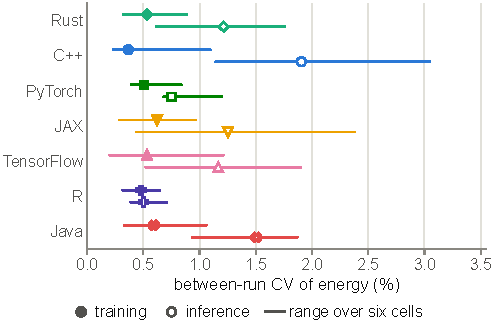
\includegraphics{figures/fig_repeatability.pdf}
    \caption{Between-run coefficient of variation of energy, from
    \vRepetitions{} independent runs per configuration: the median over the six
    (model, dataset) cells (marker; filled for training, hollow for inference)
    and the range over them (line).}
    \label{fig:repeatability}
\end{figure}


Differences of a few percent between ecosystems are therefore resolvable, and
the differences we report below are far larger. Low variance is a property of
the measurement, not a guarantee about the thing measured: a single run per
configuration would have produced an equally plausible-looking number.

\subsection{RQ1: Impact of ecosystems on training energy efficiency}
\label{subsec:rq1}

Figure~\ref{fig:energy_ci} and Table~\ref{tab:train_energy} report training
energy per epoch for every ecosystem and cell, at a common board-and-package boundary.

\begin{figure*}[t]
    \centering
    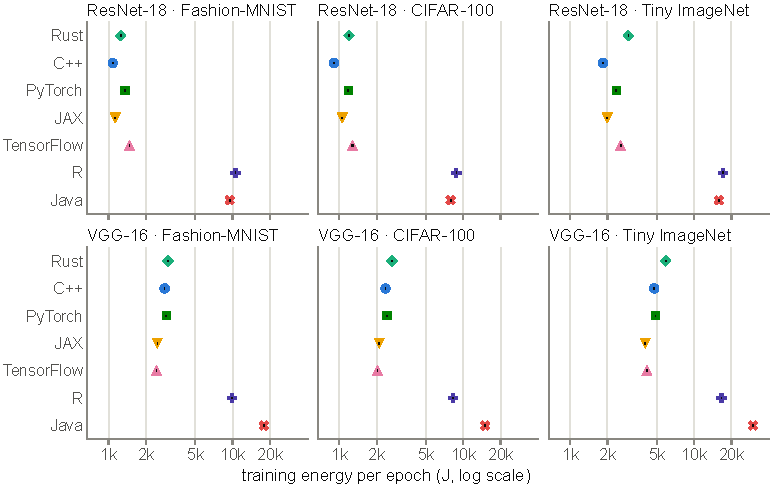
\includegraphics[width=\linewidth]{figures/fig_energy_ci.pdf}
    \caption{Training energy per epoch, accelerator plus CPU package: the mean
    over \vRepetitions{} independent runs (marker) and its 95\% Student-$t$
    interval (black line, drawn over the marker). Every interval is narrower
    than its marker. The axis is logarithmic and the same in all six panels.}
    \label{fig:energy_ci}
\end{figure*}

\begin{table*}[t]
\centering
\caption{Mean training energy per epoch (J), accelerator plus CPU package.}
\label{tab:train_energy}
\input{\gendir tab_train_energy.tex}
\end{table*}

The spread between the cheapest and the most expensive ecosystem ranges from
\vSpreadTrainMin$\times$ to \vSpreadTrainMax$\times$ depending on the cell
(Table~\ref{tab:spread}), and which stacks occupy the two ends changes with the
architecture: \vSpreadTrainBest{} is cheapest in
every ResNet-18 cell, TensorFlow in two of the three VGG-16 cells and JAX in
the third, while the most expensive is R on ResNet-18 and Java on VGG-16.
\begin{table}[t]
\centering
\caption{Cheapest and most expensive ecosystem per cell, training energy per epoch.}
\label{tab:spread}
{\footnotesize\setlength{\tabcolsep}{1.5pt}\input{\gendir tab_spread.tex}}
\end{table}


\textbf{The shared-module control group.} \vCtrlStacks{} of the
\vEcosystems{} ecosystems --- Python/PyTorch, C++ and Rust --- load the same
exported TorchScript module on the same pinned LibTorch build under
specification S1, and all \vEcosystems{} run under the single precision policy
of Section~\ref{subsec:spec}. What the group controls is the model and the
backend build. It does not control everything else those three stacks do
differently, and we do not read it as though it did.

Within the control the spread is \vCtrlSpreadMin$\times$ to
\vCtrlSpreadMax$\times$ (Table~\ref{tab:libtorch_control}), against
\vSpreadTrainMin$\times$ to \vSpreadTrainMax$\times$ across all
\vEcosystems{}. On ResNet-18 the group spans
\vCtrlSpreadResnetMin$\times$--\vCtrlSpreadResnetMax$\times$ and accounts for at
most \vCtrlShareResnetMax\,\% of the log spread; on VGG-16 it spans
\vCtrlSpreadVggMin$\times$--\vCtrlSpreadVggMax$\times$ and for as little as
\vCtrlShareVggMin\,\%. On both architectures, then, most of what separates
ecosystems separates the stacks that do not share the module from the ones that
do.


An earlier version of this study read a mechanism out of this comparison ---
binding overhead, data movement and host-side dispatch --- and it was wrong: the
precision policy then reached one stack of the three and not the others
(Section~\ref{sec:tf32}), the three did not begin from identical parameters
(Section~\ref{subsubsec:collapse}), and the stacks outside the group were not
all running the same network under the name VGG-16 (\esmsec{app:control}). All
of that is fixed in the campaign reported here. What we report from
Table~\ref{tab:libtorch_control} is the spread that survives holding the model
and the backend build fixed; a black-box design of this shape cannot decompose
what is left, and we do not.

R is reported beside the control rather than inside it. It links its own
bundled LibTorch and, because the R binding cannot switch a script module
between training and evaluation mode, builds an equivalent architecture instead
of loading the shared one --- so it shares neither the build nor the module.
Including it widens the ``shared-module'' spread to
\vFamilySpreadMin$\times$--\vFamilySpreadMax$\times$, which would have been
reported as binding overhead and is not: the difference between the two columns
of Table~\ref{tab:libtorch_control} is the cost of one member that shares less
than the label claims.

\begin{table}[t]
\centering
\caption{Spread within the shared-module control group against the full spread,
per cell. The control holds the LibTorch build, the exported module and the
data pipeline fixed, and the precision policy is fixed across all
\vEcosystems{} stacks rather than only these \vCtrlStacks{}. The
LibTorch-family column adds R, which shares the lineage but neither the build
nor the module.}
\label{tab:libtorch_control}
{\footnotesize\setlength{\tabcolsep}{1.5pt}\input{\gendir tab_control.tex}}
\end{table}

\textbf{Energy at equal quality.} A fixed-budget comparison rewards a stack for
learning less. Because every ecosystem now records test accuracy per epoch, we
can check whether it is doing so. Table~\ref{tab:accuracy} reports final test
accuracy by ecosystem, architecture and dataset, with the per-cell spread
beneath it. On Fashion-MNIST all \vEcosystems{} stacks land within
\vAccBlockSpreadFashionMax{} percentage points of one another on either
architecture, which is the strongest available evidence that they are running
the same experiment --- and a check the audited campaign could not perform,
because no ecosystem wrote its accuracy to disk. We quote the per-architecture
figure deliberately: pooling ResNet-18 and VGG-16, which reach different
accuracies in opposite per-ecosystem directions, would report
\vAccSpreadFashion{} points and would be measuring the pooling rather than the
stacks. On the harder datasets the stacks separate more --- to at most
\vAccBlockSpreadTrainedMax{} points per cell, the widest cell of the same
\emph{Spread} row, with no run excluded because none collapsed
(Section~\ref{subsubsec:collapse}) --- and there the energy
comparison must be read alongside the accuracy reached rather than instead of
it: on both harder datasets the stack that reaches the highest accuracy is also
among the two most expensive to train (Table~\ref{tab:train_energy}).

\begin{table}[t]
\centering
\caption{Final test accuracy (\%) after the fixed epoch budget, per
(architecture, dataset) cell, mean over the \vRepetitions{} runs of each cell.
The \emph{Spread} row is the highest cell of a column minus the lowest, which
is the per-cell quantity the text quotes. No run is excluded from any cell:
none collapsed to chance (Section~\ref{subsubsec:collapse}).}
\label{tab:accuracy}
{\footnotesize\setlength{\tabcolsep}{3pt}\input{\gendir tab_accuracy.tex}}
\end{table}

\begin{figure*}[t]
    \centering
    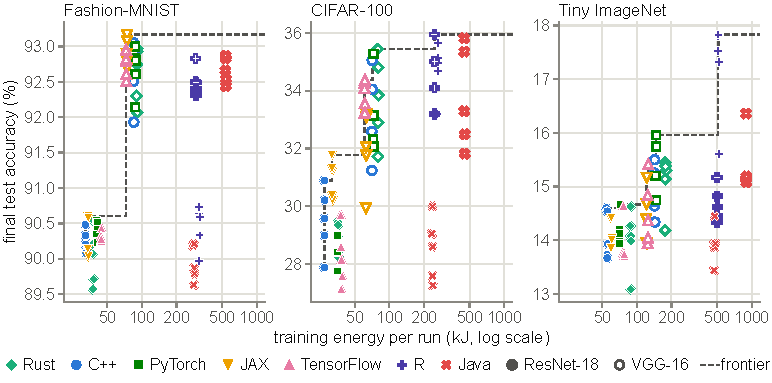
\includegraphics[width=\linewidth]{figures/fig_energy_accuracy.pdf}
    \caption{Energy spent against accuracy reached, one point per run; filled
    markers are ResNet-18 runs and hollow markers VGG-16 runs. The energy axis
    is logarithmic and the same in all three panels. The dashed line is the
    empirical frontier: no configuration to its left reaches the same accuracy
    for less energy.}
    \label{fig:energy_accuracy}
\end{figure*}


Figure~\ref{fig:energy_accuracy} plots the two together. Ranked by accuracy per
kilojoule rather than by energy alone, \vEffBest{} leads \vEffWorst{} by
\vEffRatio$\times$ --- a different quantity from the energy ratio, and closer to
the one a practitioner choosing a stack faces. Because accuracy per kilojoule
differs by two orders of magnitude between datasets we give it per dataset as
well: \vEffRatioFashion$\times$ on Fashion-MNIST, \vEffRatioCifar$\times$ on
CIFAR-100 and \vEffRatioTiny$\times$ on Tiny ImageNet, with \vEffBestFashion{},
\vEffBestCifar{} and \vEffBestTiny{} best on each. The three agree with the
pooled figure and with each other, which nothing guaranteed in advance.

\textbf{Energy to a target.} Closest of all to a practitioner's question is the
energy a stack spends before it first reaches a stated accuracy, which a
fixed-budget design cannot produce on its own (Table~\ref{tab:energy_to_target}).
On Fashion-MNIST every run of every ecosystem reaches \vTargetFashion\,\%, and
the energy to get there spans \vTargetFashionSpreadResnet$\times$ on ResNet-18,
from \vTargetFashionBestResnet{} to \vTargetFashionWorstResnet, and
\vTargetFashionSpreadVgg$\times$ on VGG-16, from \vTargetFashionBestVgg{} to
\vTargetFashionWorstVgg{} --- a like-for-like comparison at equal quality, made
within one architecture. On CIFAR-100 every run reaches \vTargetCifar\,\% as
well. On Tiny ImageNet \vTargetNeverStacksResnet{} of the \vEcosystems{} stacks
on ResNet-18, and \vTargetNeverStacksVgg{} on VGG-16, never reach
\vTargetTiny\,\% within the epoch budget; we show the empty cells, because ``did
not reach the target'' is the result. The one stack that does reach it reaches
it in every one of its runs, so its cell is a median over all \vAccRunsPerCell{}
runs; with nothing to compare it against, it is a result about that stack rather
than a comparison.

\begin{table*}[t]
\centering
\caption{Median training energy (kJ) to first reach a target accuracy, with the
number of runs that reached it where that is not all \vAccRunsPerCell{};
``never'' marks a cell in which no run reached it. Each architecture is read on
its own. Targets: \vTargetFashion\,\%, \vTargetCifar\,\%, \vTargetTiny\,\%.}
\label{tab:energy_to_target}
{\footnotesize\setlength{\tabcolsep}{3pt}\input{\gendir tab_energy_to_target.tex}}
\end{table*}


\subsubsection{Runs that consumed the budget and learned nothing}
\label{subsubsec:collapse}

In the first execution of this design \vCollapseFirstVgg{} of
\vCollapseFirstVggRuns{} VGG-16 runs \emph{collapsed}: on CIFAR-100 and Tiny
ImageNet their loss sat at $\ln N$ for the $N$ classes and their accuracy at
chance for all 30 epochs, so they consumed \vCollapseFirstWastedPct\,\% of that
campaign's training energy and learned nothing. ResNet-18 never does this in
either campaign (\vCollapsedResnet{} of \vCollapsedResnetRuns{} runs here), and
neither architecture does it on Fashion-MNIST. We had read the collapses as a
property of the ecosystems. A controlled side experiment that varied only the
initialiser --- \vInitCollapseHe{}, \vInitCollapseGlorot{} and
\vInitCollapseXavier{} collapses in \vInitCollapseTrials{} runs each under He,
Glorot and Xavier --- showed that they were the weight initialiser, which
frameworks ship differently under one architecture name. Starting every stack
from one canonical seeded export, with matched initialisers in the stacks that
build their own layers, \vCollapseRuns{} of \vCollapsedVggRuns{} VGG-16 runs
collapsed here: an exact one-sided 95\,\% upper bound of
\vCollapseRateUpperNinetyFive\,\% on the susceptible cells, against
\vCollapseFirstRateOverall\,\% measured there before, and \vWastedPct\,\% of the
\vTrainingEnergyMJ~MJ spent here went on runs that learned nothing. A per-epoch
discriminator separates collapse, where the training loss does not move, from a
pipeline defect, where it falls while test accuracy stays at chance; it found
one defect of our own on \vDefectRuns{} runs, which were deleted and
re-executed, and in the campaign as it stands it finds \vSigPipelineN{}
pipeline defects and \vSigCollapseN{} collapses. With one run per configuration,
nothing in an energy table distinguishes a collapsed run from an expensive one
(\esmsec{app:collapse}, with the first campaign's figure).

\subsubsection{The precision policy, and what it was worth}
\label{sec:tf32}

This campaign was executed twice, and the two executions differ in the
precision policy of exactly one stack: the first pinned TF32 off, with
\code{cudnn.deterministic} on, in a harness through which only Python/PyTorch
reached cuDNN, while the other six took cuDNN's Ampere default, TF32. On
\vPrecisionGapDataset{}, the one cell in which nothing else changed,
Python/PyTorch's ResNet-18 training energy is \vPrecisionPytorchRatioMin$\times$
higher with TF32 denied, while the \vPrecisionControlStacks{} comparable stacks
whose policy did not change move by at most \vPrecisionOthersMaxChangePct\,\%,
and the Python/PyTorch-versus-C++ gap that an earlier version of this study
called binding overhead falls from \vPrecisionGapBefore$\times$ to
\vPrecisionGapAfter$\times$. A kernel-level probe on a resident batch puts the
same flag pair at \vPrecisionKernelDetEnergyRatio$\times$ the accelerator energy
per step (TF32 denied alone, \vPrecisionKernelEnergyRatio$\times$; determinism
alone, \vPrecisionKernelDetOnlyRatio$\times$). PyTorch also moved from a fresh
torchvision model to the exported module between the two executions, so the
campaign ratio bounds the precision effect from above. A precision policy was
worth more here than any difference between bindings this study measures, and a
comparison that does not state its policy is not comparing ecosystems
(\esmsec{app:tf32}, with the per-cell contrast table).

\begin{tcolorbox}[colback=gray!5!white, colframe=gray!40!black, title=\textbf{RQ1 Findings: Impact of Ecosystems on Training Energy Efficiency}]
\small
Measured at a common board-and-package boundary and replicated \vRepetitions{} times
per configuration, training energy differs across ecosystems by
\vSpreadTrainMin$\times$ to \vSpreadTrainMax$\times$ depending on architecture
and dataset, with \vSpreadTrainBest{} cheapest in every ResNet-18 cell and the
cheapest VGG-16 stack changing with the dataset. Between-run
variability is small (median CV \vCVTrainMedian\,\%), so these differences are
well resolved. On Fashion-MNIST final accuracy converges to within
\vAccBlockSpreadFashionMax{} percentage points on either architecture, so there
the differences are energetic rather than qualitative. On the harder datasets the stacks do \emph{not} reach
the same accuracy --- up to \vAccBlockSpreadTrainedMax{} points on a single
(architecture, dataset) cell, with every run counted --- and there the
energy comparison must be read alongside the accuracy reached. Among the
\vCtrlStacks{} stacks that load the same exported module on the same pinned
backend build the spread is \vCtrlSpreadMin$\times$--\vCtrlSpreadMax$\times$
against \vSpreadTrainMin$\times$--\vSpreadTrainMax$\times$ across all \vEcosystems{}, so most of the
effect is between stacks that do not share a model and a backend. One cuDNN
flag was worth more than any of it: denying TF32 to a single stack cost
\vPrecisionPytorchRatioMin$\times$ its ResNet-18 training energy, which is why
a cross-ecosystem comparison that does not state its precision policy is not
comparing ecosystems.
\end{tcolorbox}

\subsection{RQ2: Impact of ecosystems on inference energy efficiency}
\label{subsec:rq2}

Table~\ref{tab:infer_energy} reports inference energy per epoch over the test
set, at the same boundary.

\begin{table*}[t]
\centering
\caption{Mean inference energy per evaluation pass (J), accelerator plus CPU package.}
\label{tab:infer_energy}
\input{\gendir tab_infer_energy.tex}
\end{table*}

The inference spread is wider than the training spread
(\vSpreadInferMin$\times$ to \vSpreadInferMax$\times$), and this is where the
apparatus matters most. An inference pass at these dataset sizes takes well
under a second in the fastest stacks, and blocks that short almost always fall
in one of the padded modes of Section~\ref{subsec:rq3}, so an inference
comparison drawn from an estimator's own duration field compares padding rather
than phases for exactly the fastest stacks. Counter-bracketing removes that
artefact but is not enough on its own, because a window measures only the work
that finishes inside it: in an earlier execution JAX's inference blocks closed
over dispatched work that had not completed, and JAX was the stack that
execution reported as cheapest at inference. The blocks here force every
asynchronous stack to completion before the window closes
(Section~\ref{sec:catalogue}). The inference phase is where a cross-ecosystem
energy study is most exposed to its instrument, and it is also the phase
practitioners deploy.

\begin{tcolorbox}[colback=gray!5!white, colframe=gray!40!black, title=\textbf{RQ2 Findings: Impact of Ecosystems on Inference Energy Efficiency}]
\small
Inference energy spreads more widely across ecosystems than training energy
(\vSpreadInferMin$\times$--\vSpreadInferMax$\times$), and does so on blocks short
enough that the measurement instrument, not the ecosystem, becomes the dominant
source of error in a naive design. Reported inference rankings should be treated
as claims about the apparatus until the window over which energy was accumulated
is stated.
\end{tcolorbox}

\subsection{RQ3: Energy--time relationship across ecosystems}
\label{subsec:rq3}

The claim that ``faster is not greener'' is a claim about two measurements, and
it is only as good as the weaker of them. We therefore recompute it on
counter-bracketed durations --- the interval between the two counter reads that
bracket a phase --- rather than on any duration reported by the estimator.

On that basis, energy and time rank the configurations almost identically:
Spearman $\rho = \vRhoTrain$ for training and $\vRhoInfer$ for inference, with
\vDiscordantTrainPct\,\% and \vDiscordantInferPct\,\% of configuration pairs
discordant respectively. Those coefficients are pooled over all
\vConfigurations{} configurations, so they are partly a statement about workload
size: a bigger dataset costs both more time and more energy whatever the stack.
Within a cell and phase --- one architecture, one dataset, one phase, the
\vEcosystems{} ecosystems --- the same coefficient runs from \vCellRhoMin{} to
\vCellRhoMax{} over the \vCellRhoCells{} cell--phase pairs, so the relation is not an
artefact of pooling workloads of different size. On CodeCarbon's reported
durations, with everything else unchanged, the coefficients are
\vRhoTrainReported{} and \vRhoInferReported{}, with
\vDiscordantTrainReportedPct\,\% and \vDiscordantInferReportedPct\,\% of pairs
discordant: the reported duration weakens the inference relation and raises its
discordant share from \vDiscordantInferPct\,\% to
\vDiscordantInferReportedPct\,\%, but the relation stays positive. Within this
workload and platform, execution time is a good proxy for energy on either
duration. What the reported duration does distort is power.


\begin{figure*}[t]
    \centering
    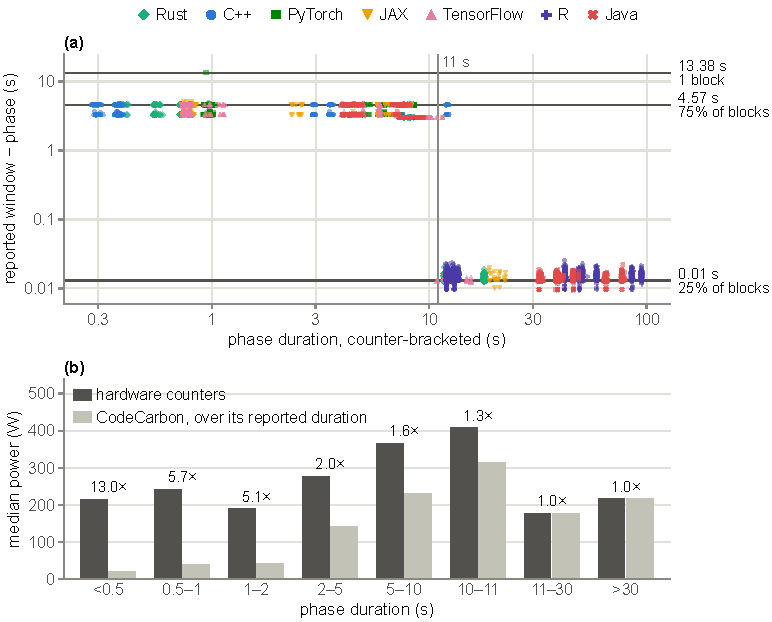
\includegraphics[width=\linewidth]{figures/fig_window_floor.pdf}
    \caption{(a) The duration reported alongside each energy figure is not the
    interval the energy was accumulated over. Each point is one block: the
    reported duration minus the counter-bracketed phase, against the phase.
    The excess falls into \vWindowModes{} discrete modes (horizontal lines,
    labelled with their median and share of blocks); the middle one holds both
    padded levels of \esmtab{tab:mechanism}, one and two network lookups
    outstanding in \texttt{stop()}, and the top one is a single block. The
    vertical line is the threshold near \vWindowThresholdS\,\si{\second}.
    (b) Median power per phase-duration bin, from the hardware counters and
    from reported energy divided by reported duration, on the bins of
    Table~\ref{tab:power_distortion}; the labels are the median factor by which
    the second understates the first. Power from the reported fields is
    understated for short phases and exact above
    \vWindowThresholdS\,\si{\second}. Both instruments are compared on the terms
    both measure.}
    \label{fig:window_floor}
\end{figure*}

Panel (a) of Figure~\ref{fig:window_floor} plots, for each block, how far the
duration CodeCarbon reports exceeds the counter-bracketed phase. The excess is not continuous:
\vWindowModeOnePct\,\% of blocks carry an excess of
\vWindowModeOneS\,\si{\second} --- that is, none --- and \vWindowModeTwoPct\,\%
carry seconds, with a median of \vWindowModeTwoS\,\si{\second}, in two
populations a second or so apart and \vWindowModeWidestS\,\si{\second} across
end to end, which the mode-finder reports as one.
\vWindowModeThreeBlocks{} of the \vBlocks{} blocks sits far above both, at
\vWindowModeThreeS\,\si{\second}. \vWindowPaddedPct\,\% of the campaign's blocks
are therefore reported with a window seconds longer than the interval over
which their energy was accumulated.

\textbf{The cause is a network call.} \texttt{EmissionsTracker.stop()} resolves
cloud metadata and then the host's geolocation over the network --- two blocking
HTTP requests --- \emph{after} the final energy reading, which is why only the
duration is affected. Both results are cached on the tracker, and a background
thread performs the same call once \vMechApiCallInterval{} measurements have
accumulated, so a block pays for however many lookups are still outstanding
when it ends. A direct probe on this host with no workload
(\esmtab{tab:mechanism}) measures the three levels: \vMechBothS\,\si{\second}
with both outstanding, \vMechOneS\,\si{\second} with one, and
\vMechNoneS\,\si{\second} for blocks longer than \vMechThresholdS\,\si{\second}.
All three appear in the campaign. A single threshold at
\vWindowThresholdS\,\si{\second} classifies \vThresholdAccuracyPct\,\% of the
\vBlocks{} blocks correctly, and every inference block is under it, and padded,
except \vWindowUnpaddedEco{}'s (\esmsec{app:rq3}). The magnitude of the padding
is network latency on this host, not a constant of the tool, and the whole
artefact is a configuration away from disappearing: an offline configuration,
or an \code{api\_call\_interval} of $-1$, removes the lookups. A study that
measures short phases with this tool and does not set that parameter will record
inflated durations, and nothing in the output says so.

The consequence for power needs no model at all.
Table~\ref{tab:power_distortion} divides each instrument's own energy by its own
duration. Below half a second the estimator's fields give
\vPowerReportedWorstW\,W where the counters measure
\vPowerMeasuredWorstW\,W, a factor of \vPowerUnderstatedWorst. The distortion falls monotonically with block length and reaches unity above
\vWindowThresholdS\,\si{\second}, where the reported window is the accumulation window and the two
agree exactly. Both sides of that comparison are the terms the two instruments
both measure; putting CodeCarbon's total in the numerator instead would mix this
artefact with the modelled RAM term criticised in Section~\ref{sec:instrument},
and did, in an earlier version of this table. The
shortest phase in the campaign takes \vShortestPhaseS\,\si{\second} and is filed
as \vShortestPhaseReportedS\,\si{\second}, a factor of \vShortestPhaseFactor.

\begin{table}[t]
\centering
\caption{Power derived from the estimator's own energy and duration fields
against power from the counters, by phase length. No model is fitted: each
instrument is divided by itself, on the terms both of them measure. The last
column is the median of the per-block ratios, not the quotient of the two
medians beside it.}
\label{tab:power_distortion}
{\footnotesize\setlength{\tabcolsep}{3pt}\input{\gendir tab_power_distortion.tex}}
\end{table}


Panel (b) plots the same quantity per block. The bias is neither random nor
uniform but monotone in phase length, so it falls hardest on the fastest
ecosystems and on the inference phase, stretching their apparent time axis while
leaving their energy untouched: that is how a study can obtain a misleading
power comparison from correct energy measurements. It does not reverse the
energy--time ranking, which on the reported durations weakens for inference and
stays positive.

\begin{tcolorbox}[colback=gray!5!white, colframe=gray!40!black, title=\textbf{RQ3 Findings: Energy and Time}]
\small
On counter-bracketed durations, energy and execution time rank the campaign's
\vConfigurations{} configurations almost identically ($\rho = \vRhoTrain$
training, $\vRhoInfer$ inference): within this
workload, faster \emph{is} greener. On the estimator's reported durations the
relation weakens for inference ($\rho = \vRhoInferReported$) but does not
reverse, so we do not reproduce the contrary finding as an artefact. What the
estimator's duration field does distort is power: it pads
\vWindowPaddedPct\,\% of blocks with seconds of tracker lifetime that carry no
energy, inflating the apparent runtime of the shortest block by
\vShortestPhaseFactor$\times$ and understating derived power by up to
\vPowerUnderstatedWorst$\times$, most for the fastest stacks.
\end{tcolorbox}

\subsection{RQ4: How much of this is the apparatus?}
\label{sec:instrument}

Every block in the campaign carries two energy readings taken over the same
phase boundaries. Figure~\ref{fig:instrument} and Table~\ref{tab:instrument} report
what they say about each other.

\begin{figure*}[t]
    \centering
    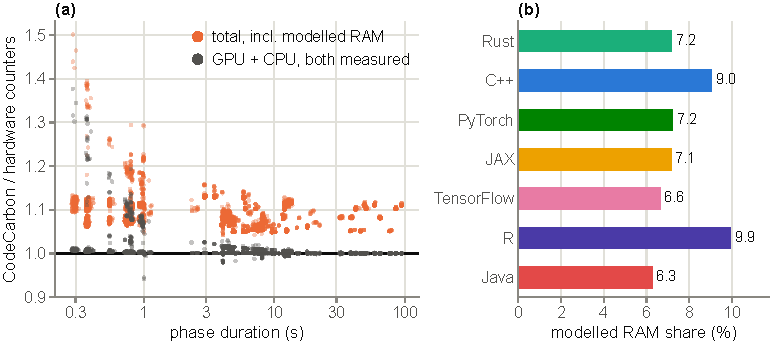
\includegraphics[width=\linewidth]{figures/fig_instrument.pdf}
    \caption{(a) Ratio of CodeCarbon to hardware counters, per block, against
    phase duration, for the GPU and CPU terms both measure (grey) and for
    CodeCarbon's total (orange). The measured part agrees; the total does not,
    by exactly the modelled RAM term. (b) The share of each ecosystem's
    reported total that is modelled RAM, mean over its blocks.}
    \label{fig:instrument}
\end{figure*}

\begin{table*}[t]
\centering
\caption{Agreement between the two readings over \vBlocks{} blocks. The mean is
over per-block ratios and is dominated by the short blocks, which carry a fixed
offset; the campaign-weighted column is the ratio of the two totals. The first
three rows compare registers with themselves.}
\label{tab:instrument}
{\footnotesize\input{\gendir tab_instrument.tex}}
\end{table*}

\textbf{On energy, the two readings agree --- and it is important to say why.}
Over the whole campaign the ratio of CodeCarbon to counters is \vCCgpuRatio{}
for the accelerator and \vCCcpuRatio{} for the CPU package, or \vCCmeasRatio{}
for their sum, a mean per-block disagreement of \vCCmeasDisagreementPct\,\%;
weighted by energy over the campaign it is \vCCmeasWeightedPct\,\%.

We initially read that as an accuracy result and it is not one. Where both
counters are exposed, CodeCarbon reads \emph{the same registers we do}: NVML's
accumulated-energy register on the accelerator and the RAPL \texttt{energy\_uj}
files on the CPU package. The two are not independent instruments; they are two
readers of one instrument. The evidence is in the residual itself. The
accelerator terms differ by a median of \vOffsetGpuMedianMJ\,\si{\milli\joule}
--- floating-point noise on the same integer register --- and essentially all of
the residual is the CPU term, a near-constant \vOffsetCpuMedianJ\,\si{\joule}
per block whose correlation with block duration is \vOffsetDurationCorr. That
constant is the counter reads being nested immediately inside the tracker's own
window rather than coinciding with it: at this machine's package power it
corresponds to a window a few milliseconds wider, and it does not grow with the
block.


This does not certify the estimator's accuracy against ground truth, which would
need a wall meter and which independent validation work
supplies~\citep{fischer2026groundtruthing}. What it certifies is that where the
counters are exposed the estimator's energy is not a model at all, so the
failure modes worth worrying about lie where the counters are \emph{not} exposed
and the substitution is silent, and in the fields beside the energy. The
resolution of the reference and the arithmetic of a fixed offset on short blocks
bound the per-block comparison (\esmsec{app:resolution}).

\textbf{On what is not measured, they cannot agree.} CodeCarbon's total exceeds
the counters by \vCCtotalRatio$\times$, and the excess is entirely its RAM term
--- \vCCramSharePct\,\% of its reported total on average --- which in machine
tracking mode, the mode a whole-machine study needs, is derived from installed
memory capacity rather than from memory activity: on this machine it infers
four modules from \SI{30.2}{\giga\byte} and yields a flat \SI{20}{\watt} for
every block, whatever the workload does to memory (\esmsec{app:ram}). No counter
on this platform can confirm or refute it. The number is not wrong so much as it
is not a measurement, added silently to a figure otherwise composed of
measurements, and on a host with more installed RAM it contributes more. Our
own boundary has the opposite failing: the counters omit DRAM energy
altogether. Neither is a whole-system number, and the difference between them
is not an error bar.

\textbf{The time between the phases belongs to the instrument.} Energy is
attributed only to the phases each stack brackets, and between the start of a
run's first block and the end of its last, tracked time ranges from
\vCoverageMin\,\% (\vCoverageWorstEco) to \vCoverageMax\,\%
(\vCoverageBestEco). The untracked time is the instrument holding its window
open: the gap preceding each block correlates with the reported-window excess at
$r = \vGapInstrumentR$ --- largely a contrast between padded and unpadded blocks
--- and that excess accounts for \vGapInstrumentPct\,\% of all untracked time,
so coverage follows block length rather than the ecosystem. Charging that time
to the ecosystems would charge them for the cost of being measured; per-phase
energy is the right quantity, and the spreads of Section~\ref{subsec:rq1} stand.
The untracked time is not free --- \vUntrackedHours{} hours across the campaign,
at least \vUntrackedMJ~MJ or about \vUntrackedPct\,\% of the reported energy at
the machine's idle draw --- but it is avoidable by the same configuration
parameter (\esmsec{app:coverage}, with the per-stack coverage in
\esmtab{tab:coverage}).

\textbf{Does the instrument change the answer?} We recomputed the ecosystem
ranking of each cell and phase under both readings. They agree in \vRankIdentical{} of \vRankBlocks{} cells ---
\vRankTrainIdentical{} of \vRankTrainCells{} in training and
\vRankInferIdentical{} of \vRankInferCells{} in inference --- and the
disagreements are adjacent-pair swaps, so no ecosystem moves more than one rank.
We report both phases because an earlier version of this analysis reported the
training figure alone, and in this campaign it is the weaker of the two: every
disagreement is a VGG-16 training cell, while the inference cells --- the phase
whose sub-second blocks this paper treats as the fragile one --- agree
throughout. The substantive ordering of RQ1 is therefore unchanged
--- provided energy, and not power or time derived from energy, is the quantity
being compared. Ranked by \emph{derived power}, the two readings disagree
everywhere, which is the finding of Section~\ref{subsec:rq3} restated.

\begin{tcolorbox}[colback=gray!5!white, colframe=gray!40!black, title=\textbf{RQ4 Findings: The Apparatus}]
\small
Over \vBlocks{} doubly instrumented blocks, a widely used software estimator
agrees with hardware energy counters to \vCCmeasDisagreementPct\,\% on the
quantity both measure --- because on this platform it is reading the same two
registers, not estimating. That is the useful finding: where the counters are
exposed, the estimator's energy is not the risk. The risks are the terms beside
it. A modelled RAM term contributes \vCCramSharePct\,\% of the reported total,
which no counter can check. \vWindowPaddedPct\,\% of blocks are reported with a
duration seconds longer than the interval their energy was accumulated over, so
power derived from those two fields is understated by up to
\vPowerUnderstatedWorst$\times$. Both produce plausible numbers; neither is
visible from the estimator's output alone. The ecosystem ranking is nonetheless
unchanged in \vRankIdentical{} of \vRankBlocks{} cells ---
\vRankInferIdentical{} of \vRankInferCells{} at inference and
\vRankTrainIdentical{} of \vRankTrainCells{} in training, where the
disagreements are adjacent-pair swaps.
\end{tcolorbox}

\subsection{The accelerator-saturation cell}
\label{sec:saturation}


At $32\times32$ per-sample compute is small. Over the training blocks
\vSatRefUtilVggHighCount{} of the \vEcosystems{} stacks hold the accelerator at
or above \vSatRefUtilHighPct\,\% utilisation on VGG-16, within
\vSatRefUtilVggMin--\vSatRefUtilVggMax\,\%, but \vSatRefUtilResnetHighCount{} on
ResNet-18, within \vSatRefUtilResnetMin--\vSatRefUtilResnetMax\,\%;
\vSatRefUtilMinEco{} is the least loaded stack on both, and the median over the
\vSatUtilCells{} (ecosystem, architecture) pairs is \vSatRefUtilMedian\,\%.
Where the GPU is lightly loaded a study may be measuring host-side work ---
decode, collation, dispatch, binding --- and calling it the energy cost of deep
learning; if so, the ecosystem spread should compress when per-sample compute
rises. We measured that in the one contrast cell the specification declares
(S7): the same \vSatEcosystems{} stacks, architectures, harness and instruments,
on Imagenette at $224\times224$ with batch 32, \vSatRuns{} runs. The cell
changes resolution, batch size and dataset together, so it measures the joint
effect of a heavier per-sample workload and not of accelerator loading alone. It
is not a fifth research question and is not pooled with the campaign; every
quantity below is computed on one definition on both sides, and
Table~\ref{tab:saturation} carries them. \esmsec{app:saturation} gives this
section's analyses in full.

\input{\gendir tab_saturation.tex}


\textbf{The cell loads the accelerator.} On the 1\,Hz \texttt{nvidia-smi} record
over each run's training blocks, the median over the cell's (ecosystem,
architecture) pairs is \vSatUtilMedian\,\%, from \vSatUtilMin\,\%
(\vSatUtilMinEco, \vSatUtilMinModel) to \vSatUtilMax\,\% (\vSatUtilMaxEco,
\vSatUtilMaxModel), against \vSatRefUtilMin\,\% (\vSatRefUtilMinEco) to
\vSatRefUtilMax\,\% (\vSatRefUtilMaxEco) at $32\times32$; per pair the median
gain is \vSatUtilGainMedian{} points. Two stacks fall well short of saturation:
Rust on ResNet-18 does not rise at all, and R remains the least loaded stack on
both architectures, at the specification's \vSatLoaderThreads{} loader workers,
which we did not vary. Every stack learned: the lowest single run of the cell
(\vSatAccRunMinEco, \vSatAccRunMinModel) ends at \vSatAccRunMin\,\% test
accuracy over ten classes.

\begin{figure*}[t]
    \centering
    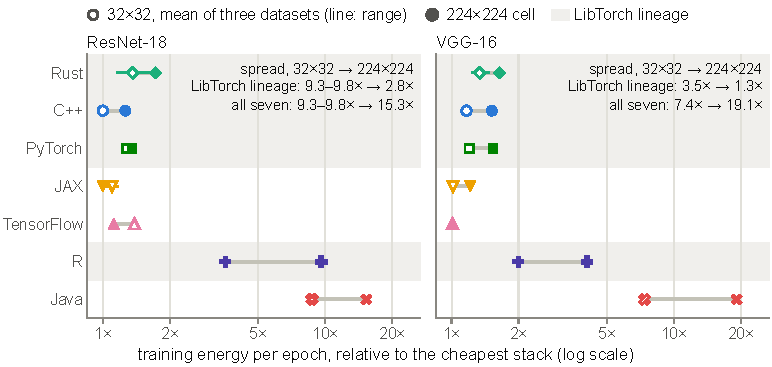
\includegraphics[width=\linewidth]{figures/fig_saturation.pdf}
    \caption{Per-epoch training energy of each stack as a multiple of the
    cheapest of the seven in the same regime: at $32\times32$ (hollow; the mean
    over Fashion-MNIST, CIFAR-100 and Tiny ImageNet, each normalised to its own
    cheapest stack, with their range as a coloured line where it is wider than
    the marker) and in the saturation cell at $224\times224$, batch 32, on
    Imagenette (filled). A stack's energy in a regime is the mean over its runs
    of the run's mean per-epoch counter energy, the definition behind the spread
    rows of Table~\ref{tab:saturation}. On the logarithmic axis the distance
    between two stacks is the spread between them. Shaded rows are the LibTorch
    lineage. The cell changes resolution, batch size and dataset together.}
    \label{fig:saturation}
\end{figure*}


\textbf{Within the LibTorch lineage the spread compresses.} The four stacks that
descend from LibTorch --- PyTorch, C++, Rust and R --- spread by
\vSatLibtorchRefSpreadTrainResnetMin$\times$--\vSatLibtorchRefSpreadTrainResnetMax$\times$
in ResNet-18 training over the three $32\times32$ datasets and by
\vSatLibtorchSpreadTrainResnet$\times$ at $224\times224$; on VGG-16, by
\vSatLibtorchRefSpreadTrainVggMax$\times$ and \vSatLibtorchSpreadTrainVgg$\times$
(Figure~\ref{fig:saturation}). Inference compresses further, and the
accelerator-only spread at $224\times224$ is of the same size. The compression
has one author: C++ is the cheapest member of the four and R the dearest for
every architecture and phase at both resolutions, so the family's spread is R's
distance from C++, and that is the distance that closes --- consistent with a
host-side share in R's cost, which the cell does not decompose. The
\vCtrlStacks{} stacks of the control group do not compress in training, where
their spread was small to begin with.

\textbf{Across all \vSatEcosystems{} the spread widens.} Training energy spreads
by \vSatSpreadTrainResnet$\times$ on ResNet-18 and \vSatSpreadTrainVgg$\times$
on VGG-16, against
\vSatRefSpreadTrainResnetMin$\times$--\vSatRefSpreadTrainResnetMax$\times$ and
\vSatRefSpreadTrainVggMax$\times$ at $32\times32$; the accelerator-only spread
is \vSatSpreadGpuTrainResnet$\times$ and \vSatSpreadGpuTrainVgg$\times$, so the
widening is not a host-side term. The dearest stack for every architecture and
phase in the cell is \vSatWorstTrainResnet{}. Setting Java aside, the other six
spread by \vSatNoJavaSpreadTrainResnet$\times$ and
\vSatNoJavaSpreadTrainVgg$\times$ in training, against
\vSatNoJavaRefSpreadTrainResnetMin$\times$--\vSatNoJavaRefSpreadTrainResnetMax$\times$
and
\vSatNoJavaRefSpreadTrainVggMin$\times$--\vSatNoJavaRefSpreadTrainVggMax$\times$
at $32\times32$: without Java the spread compresses, as it does within the
LibTorch lineage; inference is mixed. Java is the stack that reaches no cuDNN
kernel (Section~\ref{subsec:spec}), and at $224\times224$ its accelerator is
busy on both architectures, so its cost in the cell is device work rather than
host waiting --- consistent with a convolution path without cuDNN being what
separates it from the other six, but not a measurement of it: the
\vCudnnOffEnergyRatio$\times$ bound was taken at $32\times32$ and we did not
repeat it at $224\times224$.

\textbf{The ordering partly survives.} Over \vSatRankComparisons{} comparisons
of the $224\times224$ ordering with that on each $32\times32$ dataset (exact
permutation $p$, since seven items give only $7!$ orderings), VGG-16 training
keeps its order or nearly: $\rho = \vSatRankRhoTrainVggCifar$,
\vSatRankRhoTrainVggFashion{} and \vSatRankRhoTrainVggTiny{} against CIFAR-100,
Fashion-MNIST and Tiny ImageNet. ResNet-18 training and inference on both
architectures agree more weakly ($\rho$ down to \vSatRankRhoMin, $p$ up to
\vSatRankPermMax). What moves is the top: \vSatRefBestTrainResnet{}, the
cheapest ResNet-18 stack in training on every $32\times32$ dataset, is not the
cheapest at $224\times224$, where it is \vSatBestTrainResnet{} on ResNet-18 and
\vSatBestTrainVgg{} on VGG-16, and in a single comparison up to
\vSatRankMovedMax{} stacks move by two places or more. A ranking read off the
campaign is a statement about its regime.

\textbf{Faster is still greener.} On the definition behind RQ3, run time and run
energy rank the cell's \vSatRhoCells{} (ecosystem, architecture) pairs at $\rho
= \vSatRhoTrain$ in training and \vSatRhoInfer{} in inference, against
\vSatRefRhoTrain{} and \vSatRefRhoInfer{} over the campaign's configurations;
\vSatDiscordantTrainPct\,\% and \vSatDiscordantInferPct\,\% of pairs are
discordant. With the accelerator loaded, mean training board power sits between
\vSatPowerCounterMin\,\si{\watt} and \vSatPowerCounterMax\,\si{\watt} across the
cell, a range far narrower than that of run time (Table~\ref{tab:saturation}),
so time remains the larger factor in energy.

\begin{tcolorbox}[colback=gray!5!white, colframe=gray!40!black, title=\textbf{Saturation-cell Findings: Does the Spread Survive a Heavier Workload?}]
\small
At $224\times224$ and batch 32, where median training-block utilisation is
\vSatUtilMedian\,\%, the ecosystem spread does not collapse: across all
\vSatEcosystems{} stacks training energy spreads by
\vSatSpreadTrainResnet$\times$ (ResNet-18) and \vSatSpreadTrainVgg$\times$
(VGG-16), wider than at $32\times32$. Within the LibTorch lineage it compresses
to \vSatLibtorchSpreadTrainResnet$\times$ and \vSatLibtorchSpreadTrainVgg$\times$,
because R, the stack that leaves the accelerator least loaded, closes most of
its distance from C++;
without Java the other six compress too, to
\vSatNoJavaSpreadTrainResnet$\times$ and \vSatNoJavaSpreadTrainVgg$\times$.
The widening comes from Java, the one stack that reaches no cuDNN kernel and
whose cost in the cell is device work; we did not bound the missing backend's
share at this resolution. The VGG-16 training order is preserved, the cheapest
stacks change, and faster is still greener ($\rho = \vSatRhoTrain$ training,
\vSatRhoInfer{} inference).
\end{tcolorbox}

\section{Discussion}
\label{sec:discussion}


The energy efficiency of DL workloads is materially influenced by the
\emph{choice of language--framework
ecosystem}~\citep{georgiou2022green,marini2025green,pereira2021ranking,gordillo2024ranking}.
This section interprets that result and draws lessons for different
stakeholders.

\subsection{Interpretation of Results}
\label{subsec:interpretation}

\textbf{The ecosystem effect is large, and most of it is between stacks that
share nothing but the specification.} Fixing the model and the backend build
removes most of the training spread on both architectures
(Table~\ref{tab:libtorch_control}); what remains sits between frameworks rather
than inside one backend, and nothing in a black-box design of this shape
decomposes it. The absolute gap widens with dataset size and with per-sample
compute, so the choice matters most exactly where energy does. Runtime layers,
input pipelines, execution engines and toolchains all differ, so these are
ecosystem-level effects, not effects of a programming language.

\textbf{The phases rank ecosystems similarly but not identically, and an
estimator-based analysis exaggerates the difference.} On counter-bracketed
energy the same ecosystem is cheapest in both phases in \vPhaseSameBest{} of
\vPhaseBlocks{} cells and the full ordering is identical in
\vPhaseIdenticalOrder{} of them, with Spearman correlations between each cell's
training and inference energies of \vPhaseRhoMin{} to \vPhaseRhoMax. The
opposite claim --- that the phases rank differently and so demand phase-aware
stack selection --- is a natural conclusion to draw from estimator output,
because almost all inference blocks fall in one of the padded modes of
Section~\ref{subsec:rq3}, so an inference ranking derived from an estimator's
own duration is partly a ranking of padding. We do not claim phase-dependence
never occurs; establishing it requires an instrument whose window is known.

\textbf{Faster \emph{is} greener, here.} This contradicts a well-established
finding in cross-language energy
work~\citep{weber2023twins,rua2024large,pereira2021ranking}, and the scope of the
contradiction matters. Those studies largely concern CPU-bound general-purpose
benchmarks, where a language can trade instruction count against memory traffic
and shift energy per second substantially. In a GPU-bound DL workload the
accelerator dominates and runs in a narrow band of power, so time and energy are
nearly proportional almost by construction. We report a scope condition on the
established finding, not a refutation of it.

\textbf{Quality must be measured, not assumed.} An efficiency claim on the
harder datasets that does not report accuracy alongside energy compares stacks
that did different amounts of learning, and an ecosystem that converges more
slowly looks efficient precisely because it accomplished less. Here the
corrected and uncorrected figures coincide --- \vAccSpreadCifar{} points on
CIFAR-100 pooled over both architectures, either way --- because no run
collapsed (Section~\ref{subsubsec:collapse}). In the campaign this one replaces
they did not coincide, and the difference was runs at chance accuracy averaged
in as though they were measurements.

\subsection{Implications for Stakeholders}

\begin{itemize}
 \item \textbf{Researchers:} report energy alongside accuracy, and both
 alongside the measurement boundary. Our stronger recommendation is procedural:
 a cross-stack study needs a written specification and a mechanism that enforces
 it, because every divergence we corrected produced a plausible number first and
 most were caught by a mechanism rather than by inspection
 (Section~\ref{sec:catalogue}).

 \item \textbf{Practitioners:} ecosystem choice has a first-order effect on
 energy; because the phases rank stacks similarly but not identically, a
 phase-specific split needs its own measurement. Efficiency must be weighed
 against maintainability, hiring, library availability and time to delivery: an
 energy gap of this size is not a mandate when the cheaper stack has a tenth of
 the ecosystem around it.

 \item \textbf{Framework and tool designers:} the target we can name is the
 convolution backend: Deeplearning4j's final release reaches no cuDNN path, and
 losing cuDNN can cost up to \vCudnnOffEnergyRatio$\times$ the energy
 (Section~\ref{subsec:spec}). Measurement tools should report the interval over
 which energy was accumulated, and fail rather than substitute a model when a
 counter is unavailable: an instrument that refuses to run is more useful than
 one that quietly estimates.

 \item \textbf{Policy makers and funding agencies:} AI efficiency is
 multi-dimensional, and adopting any single metric as a target invites
 Goodhart's Law. Reporting requirements should ask for the measurement boundary
 and the replication count, not only the number: a figure without either is not
 auditable, and our own experience is that unauditable figures are wrong more
 often than not.
\end{itemize}

\subsection{AI Requires Explicit Energy Measurement}
\label{sec:explicit_measurement}

Ecosystem selection is not a neutral engineering choice: it shifts DL energy
consumption by a factor that is large and reproducible across repetitions of the
same configuration. How wide that factor is depends on where the measurement
boundary is drawn, and the choice is not visible in the resulting number. The
audited campaign shows this on its own records, without any comparison across
machines: its ecosystem spread is \vAuditSpreadConfounded$\times$ when energy is
taken as the estimator's total and \vAuditSpreadGpuOnly$\times$ when it is taken
as the estimator's accelerator term alone. Both come from the same instrument;
a constant host term added to every stack compresses their ratios toward one, so
widening the boundary narrows the apparent effect without changing anything that
was measured. Any cross-ecosystem ratio is therefore a statement about a
boundary as much as about the stacks.

Establishing the result is harder than it looks: every defect we found
produced numbers of the right magnitude, units and relative ordering, and was
detectable only by a second instrument, an executable specification, or a
quality metric the study happened to record. We therefore make the artefacts
as important as the findings. The specification, the measurement contract, the
conformance checker and the raw dual-instrument records are in the replication
package, and the manuscript's numbers are generated from them; a reader who
doubts a figure can regenerate it, and one who doubts the apparatus can run the
checks. Translating the measured multipliers into hyperscale energy and cost is
a projection rather than a measurement, so it is in \esmsec{sec:scenario}.

\section{A catalogue of defect classes}
\label{sec:catalogue}

Auditing the earlier eight-stack campaign and repairing every stack against the
specification turned up \vDefectCount{} defect \emph{classes}: plausible
mistakes in any study of this shape, several of them language or tool
\emph{defaults} rather than oversights, and most invisible in the resulting
measurements. \esmsec{app:catalogue} lists every class with its
measured effect and whether a reader given only the released data could detect
it. The classes fall in four groups: the \emph{instrument} (what is read ---
a unit mislabelled by a factor of \(3.6\times10^{6}\), a padded duration, a
modelled term in a measured total, mixed tracker versions and modes, device
work outliving its window), the \emph{implementation} (what the stacks compute
--- divergent learning rates, loaders, input shapes, evaluation batching,
initialisers and seeds, four networks under one name; two of the audited
campaign's stacks trained at ten times the stated learning rate,
\esmtab{tab:protocol}), \emph{placement} (a silent CPU fallback, a linker
dropping the CUDA dependency) and \emph{analysis} (collapsed and partial runs
averaged in, epochs treated as replications). Only three classes are visible
from the released data; the rest require reading the code, a second
instrument, or a quality metric the study thought to record. \vDefectOurs{} of
the \vDefectCount{} are ours: most were caught by a mechanism rather than by
attention, and two by none --- one by an accelerator drawing idle power, one by
the campaign failing on its first batch with every check green. Enforcement
beats discipline, and our own discipline was not sufficient either.

\section{Threats to Validity}
\label{sec:threats}

We group threats conventionally, quantify them where the data allow, and give
the full discussion in \esmsec{app:threats}.

\textbf{This campaign replaces one of our own.} An earlier campaign of exactly
this design ran to completion and produced a coherent set of numbers; auditing
it against its own source found three headline claims confounded --- a precision
policy in force for one stack only, four different networks under the name
VGG-16, and diverging weight initialisers. We aligned the stacks and
re-executed all \vRuns{} runs, and every ecosystem comparison here is measured
after that alignment. What carries over is the apparatus: the instrument
comparison, the reported-window result, the boundary argument and the
source-level defects are statements about the tooling, each re-derived from this
campaign. A result about what the stacks did needs the stacks to have been doing
the same thing; a result about the instrument does not.

\textbf{Internal validity.} Whole-machine tracking means that concurrent work
contaminates a measurement: the host was otherwise idle, and blocks measured
during development while a download ran were discarded and the protocol
amended. Toolchain heterogeneity remains --- CUDA ranges from 11.6
(Deeplearning4j) to 12.8 (the control group) --- and cannot be removed, since an
ecosystem is partly defined by its toolchain; it is bounded by the pinned
control group and the campaign-wide precision policy, though
Table~\ref{tab:libtorch_control} does not say what the surviving spread is.
Implementation drift, the dominant internal threat in studies of this shape, is
attacked by the specification and its \vConformanceChecks{} checks, with the
residual gaps stated in Section~\ref{subsec:spec}; two of our own defects
escaped every check, so we claim only that a divergence now has to survive an
executable check, and that the campaign itself is the last check in the
sequence.

The defect catalogue names the lowest mean accelerator power among the stacks
as the signature of a stack silently running on the host, and we applied that
diagnostic to our own data. \vLowestGpuEco{} draws the lowest accelerator power, \vLowestGpuW\,\si{\watt} against up to
\vHighestGpuW\,\si{\watt} for the others on a \SI{350}{\watt} card. The CPU
term clears it: its
package power, \vLowestGpuEcoCpuW\,\si{\watt}, is inside the
\vCpuPowerAcrossMinW--\vCpuPowerAcrossMaxW\,\si{\watt} band of every other stack,
and the S4 assertion refuses a CPU device. It uses the accelerator at a low duty
cycle --- \vLowestGpuUtilResnetPct\,\% utilisation on ResNet-18 and
\vLowestGpuUtilVggPct\,\% on VGG-16 over each run's wall clock --- and its epochs
are the longest in the campaign. Accelerator placement is verified rather than
assumed: a Rust binary linked against a CUDA LibTorch runs on the CPU by
default, because \texttt{--as-needed} drops the CUDA dependency no Rust symbol
references, so the dynamic section of every Rust binary we build is checked.

\textbf{Construct validity.} Our construct is energy at a stated boundary, not
``sustainability'': accelerator board plus CPU package, excluding the power
supply, fans, drives, chipset and host DRAM. We had no wall meter, and a
board-and-package number must not be compared with a wall-meter number from
another study. The counters are not exempt from scrutiny: RAPL's package energy
is itself modelled on some parts~\citep{khan2018rapl}, and NVML rests on
internally averaged board telemetry, so for the shortest blocks both instruments
are near the edge of what they resolve --- a joint property of the pair, which
does not bear on the reported-duration finding. Two counter-side defects of ours
were fixed for this campaign: a RAPL wrap guard with the wrong units, inert for
every block but never needed (the longest block is
\vLongestBlockS\,\si{\second}), and manifests without machine state, which every
run now records. Every figure is un-baselined: on an idle host this machine
draws \vIdleTotalW\,\si{\watt} at the boundary (\vIdleGpuW\,\si{\watt} at the
accelerator, \vIdleCpuW\,\si{\watt} at the CPU package),
\vIdleShareOfBlockPct\,\% of the mean power of a measured block. The CPU term is
mostly the machine being on --- its idle draw is \vIdleCpuSharePct\,\% of its
campaign mean, against \vIdleGpuSharePct\,\% for the accelerator --- yet
contributes \vCpuShareOfTotalPct\,\% of reported energy; this boundary carries no
measured host-side term, which is one reason we do not apportion the spread
between host-side and accelerator work. The estimator's modelled RAM term and
its padded duration (Sections~\ref{subsec:rq3} and~\ref{sec:instrument}) are
construct threats to any study built on its output, and we use counter energy
and counter-bracketed durations throughout.

\textbf{External validity.} We studied two convolutional architectures on three
image classification datasets at $32\times32$, and one contrast cell at
$224\times224$; results may not generalise to other model families, to
transformers, or to other resolutions and batch sizes, where the balance between
accelerator and host-side work differs. The campaign compares whole pipelines
rather than saturated kernels, and the contrast cell shows that the stacks move
by different amounts and in different directions as that balance moves, so the
campaign's multipliers are not constants to carry to another workload. The cell
is one point: it changes resolution, batch size and dataset together, ran at
\vSatLoaderThreads{} loader workers only, and did not repeat the cuDNN bound.
The platform is a single-accelerator desktop, whose host share of energy is
smaller than a multi-socket server's, and MATLAB's absence is a conformance
limit, not a result about MATLAB.

\textbf{Conclusion validity.} Epochs within a run are not independent, so every
interval and test here is computed on \vRepetitions{} independent runs per
configuration, \vInterleavedRuns{} of the \vRuns{} runs interleaved. Five
repetitions is a small sample for a rank test, and we report what that costs. A
Kruskal--Wallis test rejects equality of ecosystems in all \vOmnibusBlocks{}
test groups ($p \le \vOmnibusMaxP$, $\varepsilon^2 \ge \vOmnibusEpsMin$), and
\vPairsLargePct\,\% of the \vPairsTotal{} pairwise comparisons carry a large
Cliff's delta --- an effect size saturated by a between-run coefficient of
variation under half a per cent, which records that groups separate, not by how
much. Yet \vPairsSignificant{} of those pairs is significant after Holm
correction, and cannot be at any effect size: with five runs against five the
smallest exact two-sided Mann--Whitney $p$ is \vPairsMinRawP, which Holm over the
\vPairsPerBlock{} comparisons within a group raises to \vPairsMinHolmP. The
design can establish that the ecosystems differ but not order any particular
pair, so the ordering claims rest on effect sizes and intervals. The first
campaign's collapse rates warranted an exact Freeman--Halton test
($p = \vCollapseFirstExactP$) rather than the $\chi^2$ and permutation tests we
first ran; on this campaign it returns $p = \vCollapseExactP$, because no
ecosystem collapsed a run. Finally, \vLateRuns{} runs (\vLateConfigurations{}
configurations, all \vLateEcosystems{}) were replayed \vLateGapDays{} days after
the rest and are not interleaved. Re-executing one completed configuration
(\vCalibConfig) in a third window bounds the drift: training energy is
\vCalibTrainDiffPct\,\% lower, \vCalibTrainSD{} within-window standard
deviations, and comparable; inference is \vCalibInferDiffPct\,\% lower,
\vCalibInferSD{} standard deviations (\vCalibInferDiffJ\,\si{\joule} per block),
which we carry as a between-window uncertainty of that order on the late
inference figures --- small against the ecosystem differences but not noise,
and obtained from one configuration in a different ecosystem.

\section{Conclusion}
\label{sec:conclusion}

This paper presented an empirical study of how \emph{language--framework
ecosystems} affect the energy efficiency of \emph{Deep Learning} workloads,
across \vEcosystems{} ecosystems, two convolutional architectures and three
datasets, replicated \vRepetitions{} times per configuration and instrumented
twice per measurement block.

Four findings stand out.

First, ecosystem selection substantially shifts operational efficiency: at a
common board-and-package boundary, training the same model on the same data costs
between \vSpreadTrainMin$\times$ and \vSpreadTrainMax$\times$ more energy on one
ecosystem than another, with between-run variability of order
\vCVTrainMedian\,\%. \vCtrlStacks{} of the ecosystems compared load the same
exported TorchScript module on the same pinned backend build, and among those
three the spread is \vCtrlSpreadMin$\times$--\vCtrlSpreadMax$\times$ against
\vSpreadTrainMin$\times$--\vSpreadTrainMax$\times$ across all \vEcosystems{}: most
of the gap is between stacks that do not share a model and a backend, and we
report that without a decomposition of the part that remains.

Second, on the easiest dataset the effect is energetic and not qualitative: all
\vEcosystems{} stacks converge to within \vAccBlockSpreadFashionMax{} percentage
points on Fashion-MNIST under the same epoch budget, doing the same work at very
different cost. That equivalence does not extend to the harder datasets, where
the stacks differ by up to \vAccBlockSpreadTrainedMax{} points on a single cell,
and where energy must therefore be read alongside accuracy rather than instead
of it.

Third --- and this is the finding we did not expect --- the apparatus decides
part of the answer, in one specific and correctable way: not the energy, on
which the two instruments agree, but the fields derived beside it.
Over \vBlocks{} doubly instrumented blocks, a widely used software estimator
agrees with hardware energy counters to \vCCmeasDisagreementPct\,\% on energy.
But the duration it reports beside that energy is not the interval the energy
was accumulated over: \vWindowPaddedPct\,\% of blocks carry seconds of tracker
lifetime in which no energy was drawn, so power derived from the two fields is
understated by up to \vPowerUnderstatedWorst$\times$ on the shortest blocks.
Recomputed on measured durations, energy and time rank the \vConfigurations{}
pooled configurations at $\rho = \vRhoTrain$ in training, and within a single
cell and phase at $\rho = \vCellRhoMin$ to \vCellRhoMax: in this workload, faster
\emph{is} greener. On the estimator's own durations the relation weakens for
inference but stays positive, so we do not reproduce the contrary result as an
instrument artefact; the artefact we do find is in derived power.

Fourth, the campaign's per-sample compute is small, and we tested whether that
is what produced the spread. In a declared contrast cell at $224\times224$ and
batch 32, which loads the accelerator for most stacks, the spread within the LibTorch
lineage compresses to \vSatLibtorchSpreadTrainVgg$\times$--\vSatLibtorchSpreadTrainResnet$\times$
in training, while across all \vSatEcosystems{} it widens to
\vSatSpreadTrainResnet$\times$--\vSatSpreadTrainVgg$\times$, carried by the one
stack without a cuDNN path; without it, the other six compress too. The
ecosystem effect survives a heavier per-sample workload; its size and its
cheapest stack do not carry over unchanged.

We draw a procedural conclusion from that. A cross-ecosystem energy study needs
a written specification, a mechanism that enforces it, and a second instrument
--- for the same reason that a performance benchmark needs a stated warm-up
policy. Every defect we corrected in building this study produced a plausible
number first. The specification, the shared measurement contract, the \vConformanceChecks{}-check
conformance checker and the raw dual-instrument records are part of the
replication package, and every figure in this paper is generated from them.

%%%%%%%%%%%%%%%%%%%%%%%%%%%%%%%%%%%%%%%%%%%%%%%%%%%%%%%%%%%%%%%%%%%%%%%%%%%%%%%
\section{Future Work}
\label{sec:future}


Several directions remain open. First, the workload should extend beyond CNNs to
transformer and multimodal architectures, whose kernels are attention and matrix
multiplication rather than convolution, and along a sweep of resolution and
batch size rather than at two points; a cuDNN-off bound at $224\times224$ would
settle how much of Java's distance at saturation its missing convolution backend
accounts for. Second, heterogeneous hardware --- server-class accelerators,
TPUs, edge devices --- would establish how much of the ranking is a property of
the stacks and how much of this host (a server-class accelerator saturates at a
different point from the desktop card the saturation cell loads), treating the hardware--software stack as
part of the ecosystem rather than as a nuisance parameter. Third, a white-box
layer would localise where the \vCtrlSpreadMin$\times$--\vCtrlSpreadMax$\times$
that survives a fixed model, data and backend build originates: loader
scheduling, host-to-device transfer, launch overhead and allocator behaviour on
one side, kernel selection, algorithm choice and precision policy on the other.
Fourth, the reported-window padding of one estimator on one platform invites
replication across estimators, sampling intervals and tracking modes, and the
method --- bracket every block with hardware counters and compare --- is cheap.
Finally, a wall-meter reference would relate our board-and-package boundary to
the whole-system energy an operator pays for.

%%%%%%%%%%%%%%%%%%%%%%%%%%%%%%%%%%%%%%%%%%%%%%%%%%%%%%%%%%%%%%%%%%%%%%%%%%%%%%%

\section{Carbon Footprint of This Study}

The campaign reported here consumed \vCampaignEnergyMJ~MJ
(\vCampaignEnergyKWh~kWh) at the accelerator and CPU package across \vRuns{}
runs. At the grid carbon intensity CodeCarbon assigns to this location, that
corresponds to a few kilograms of CO$_2$e --- modest against industrial
training, and reported here for the same reason we ask others to report it: an
energy figure without a stated boundary and a stated scope is not auditable.
The figure above is the energy inside the measured blocks. It excludes
development, failed runs and the two earlier campaigns of this design, one of
them on other hardware and at another boundary --- including those would make it
several times larger --- and it excludes the machine's draw
during the untracked time between blocks discussed in
Section~\ref{sec:instrument}, a further \vUntrackedMJ~MJ. An honest campaign-level
figure is therefore larger than the one we report and we do not pretend
otherwise; what we report is the quantity the comparisons are made on.

The saturation cell of Section~\ref{sec:saturation} is reported separately,
because nothing in this paper pools it with the campaign. Its \vSatRuns{} runs
consumed \vSatCampaignEnergyMJ~MJ (\vSatCampaignEnergyKWh~kWh) inside their
measured blocks, at the same boundary and on the same definition as the figure
above. The same exclusions apply to it --- development, failed runs and the time
between blocks --- and we have not measured
the untracked share for the cell, so its campaign-level figure is likewise
larger than the one we report.

